% Created 2021-04-20 Tue 19:43
% Intended LaTeX compiler: pdflatex

\documentclass[english]{article}
\usepackage[T1, T2A]{fontenc}
\usepackage[lutf8]{luainputenc}
\usepackage[english, russian]{babel}
\usepackage{minted}
\usepackage{graphicx}
\usepackage{longtable}
\usepackage{hyperref}
\usepackage{xcolor}
\usepackage{natbib}
\usepackage{amssymb}
\usepackage{stmaryrd}
\usepackage{amsmath}
\usepackage{caption}
\usepackage{mathtools}
\usepackage{amsthm}
\usepackage{tikz}
\usepackage{grffile}
\usepackage{extarrows}
\usepackage{wrapfig}
\usepackage{algorithm}
\usepackage{algorithmic}
\usepackage{lipsum}
\usepackage{rotating}
\usepackage{placeins}
\usepackage[normalem]{ulem}
\usepackage{amsmath}
\usepackage{textcomp}
\usepackage{capt-of}


\usepackage{geometry}
\geometry{a4paper,left=2.5cm,top=2cm,right=2.5cm,bottom=2cm,marginparsep=7pt, marginparwidth=.6in}
 \usepackage{hyperref}
 \hypersetup{
     colorlinks=true,
     linkcolor=blue,
     filecolor=orange,
     citecolor=black,      
     urlcolor=blue,
     }

\date{}
\title{}
\hypersetup{
 pdfauthor={},
 pdftitle={},
 pdfkeywords={},
 pdfsubject={},
 pdfcreator={Emacs 28.0.50 (Org mode 9.4.4)}, 
 pdflang={English}}
\begin{document}

\begin{titlepage}
  \begin{center}
    \large\textbf{Федеральное государственное автономное образовательное учреждение высшего образования ``Национальный исследовательский университет ИТМО``} \\
    \vspace{0.5cm}
    Факультет информационных технологий и программирования \\
    \vspace{0.5cm}
    Направление ``Прикладная математика и информатика`` \\
    \vspace{3cm}
    Отчет к лабораторной работе №4 \\
    \vspace{0.5cm}
    \textbf{Изучение алгоритмов метода Ньютона и его модификаций}
  \end{center}
  \vfill
  \begin{flushright}
    \large
    Выполнили студенты группы М3237 \\
    \vspace{0.5cm}
    Ярошевский Илья \\
    Аникина Вероника \\
    Крюков Александр
  \end{flushright}
  \vspace{3cm}
  \begin{center}
    Санкт-Петербург 2021
  \end{center}
\end{titlepage}
\section{Цели работы}
Реализовать и ислледовать:
\begin{itemize}
\item методы Ньютона:
  \begin{itemize}
  \item классический
  \item с одномерным поиском
  \item с направлением спуска
  \end{itemize}
\item метод Бройдена-Флетчера-Шено и метод Пауэлла
\item метод Марквардта двумя вариантами
\end{itemize}
\section{Ход работы}
\subsection{Методы Ньютона}
\subsubsection{Схема работы}
Особенность данных, а также всех последующих, методов в том, что они
используют возможность вычисления Гессиана \(H(\vec{x})\)
функции. Направление спуска в общем виде определяется как решение СЛАУ
\[ H(x)p^k = -\nabla f(x^{k - 1}) \]
Для решения СЛАУ использовался метод Гаусса с выбором главного элемента
\subsubsection{Исследование на функциях}
\begin{enumerate}
\item
  \[ f_1(\vec{x}) = \frac{1}{2} \left\langle \begin{pmatrix} 2 & -1 \\ -1 & 1 \end{pmatrix} x, x \right\rangle + \langle \begin{pmatrix} 2 & -3 \end{pmatrix} , x \rangle + 10 \]
  \[ x_0 = \begin{pmatrix}
    1 & 1
    \end{pmatrix} \]
  \begin{center}
    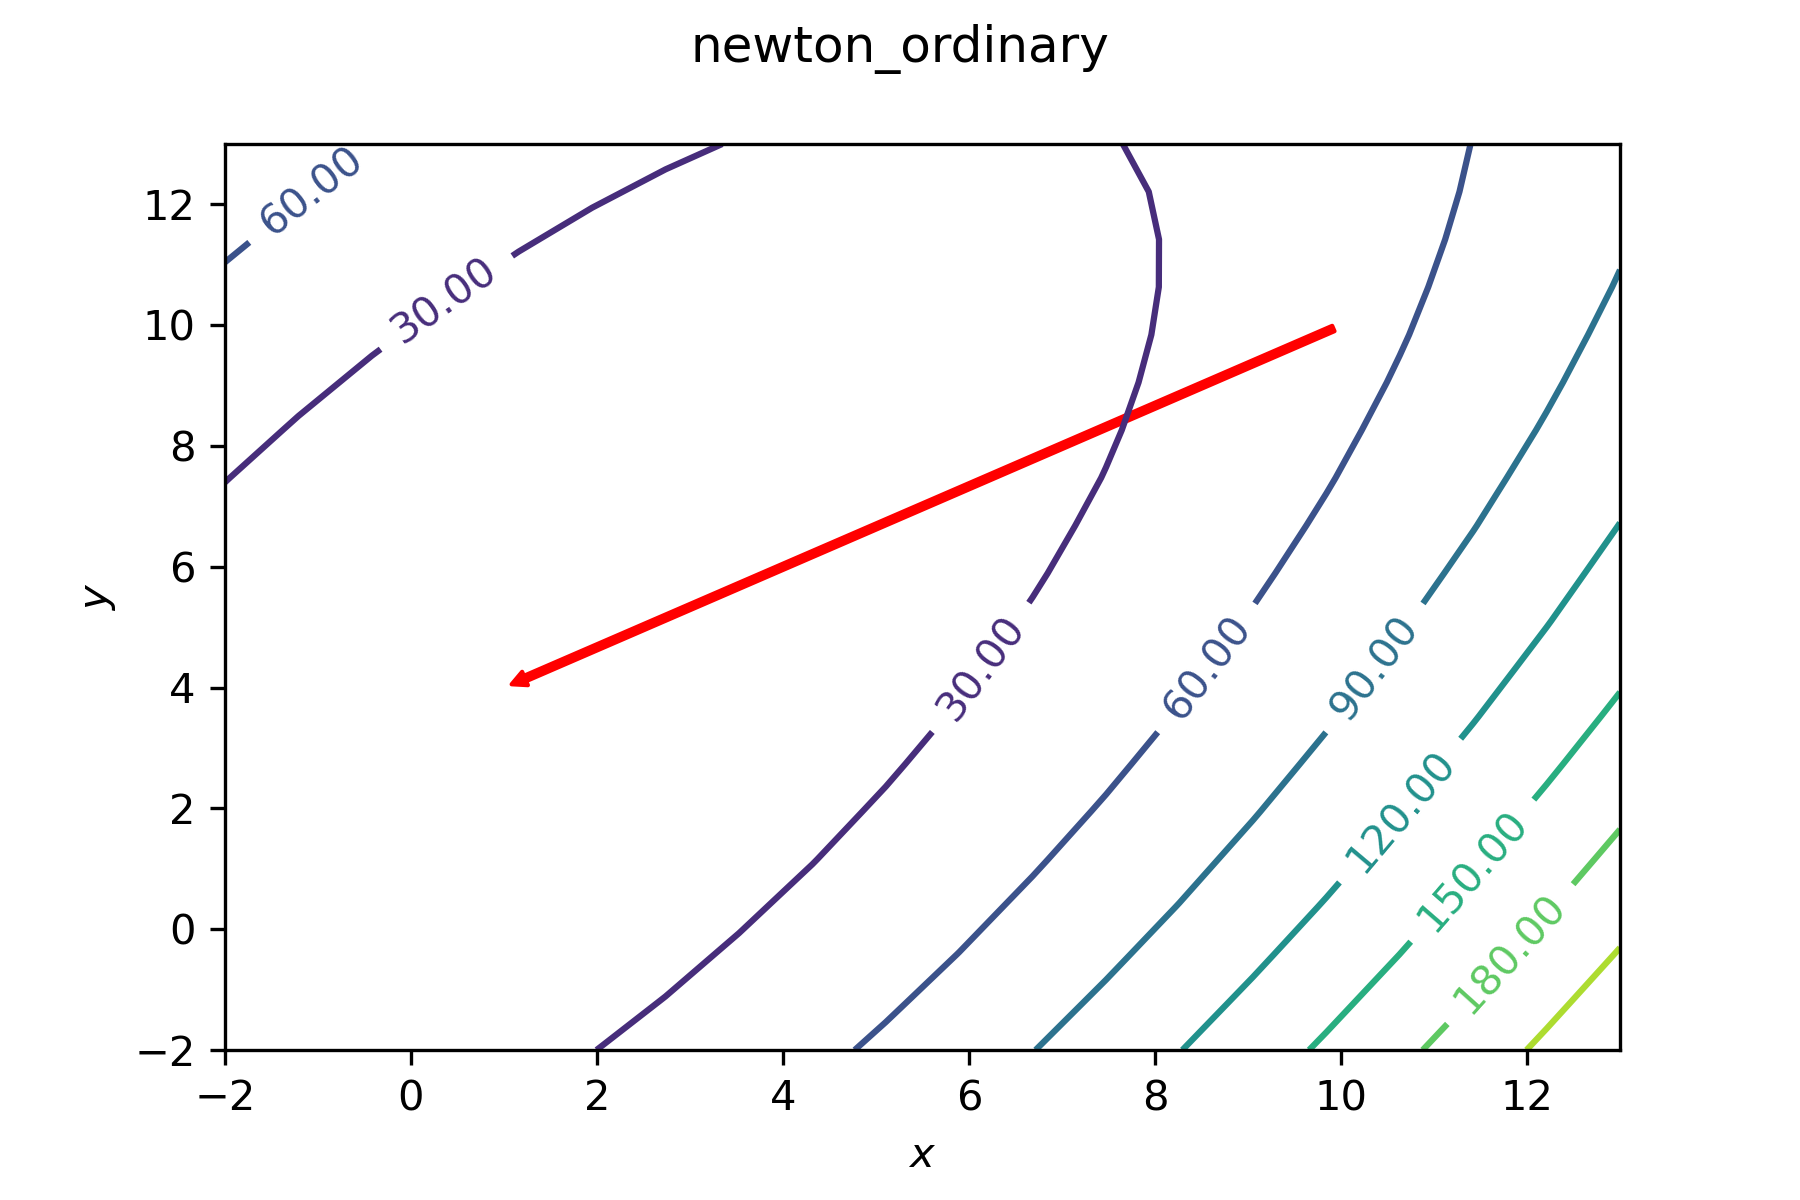
\includegraphics[scale=0.7]{plots/contours_newton_ordinary_1.png}
  \end{center}
  \begin{center}
    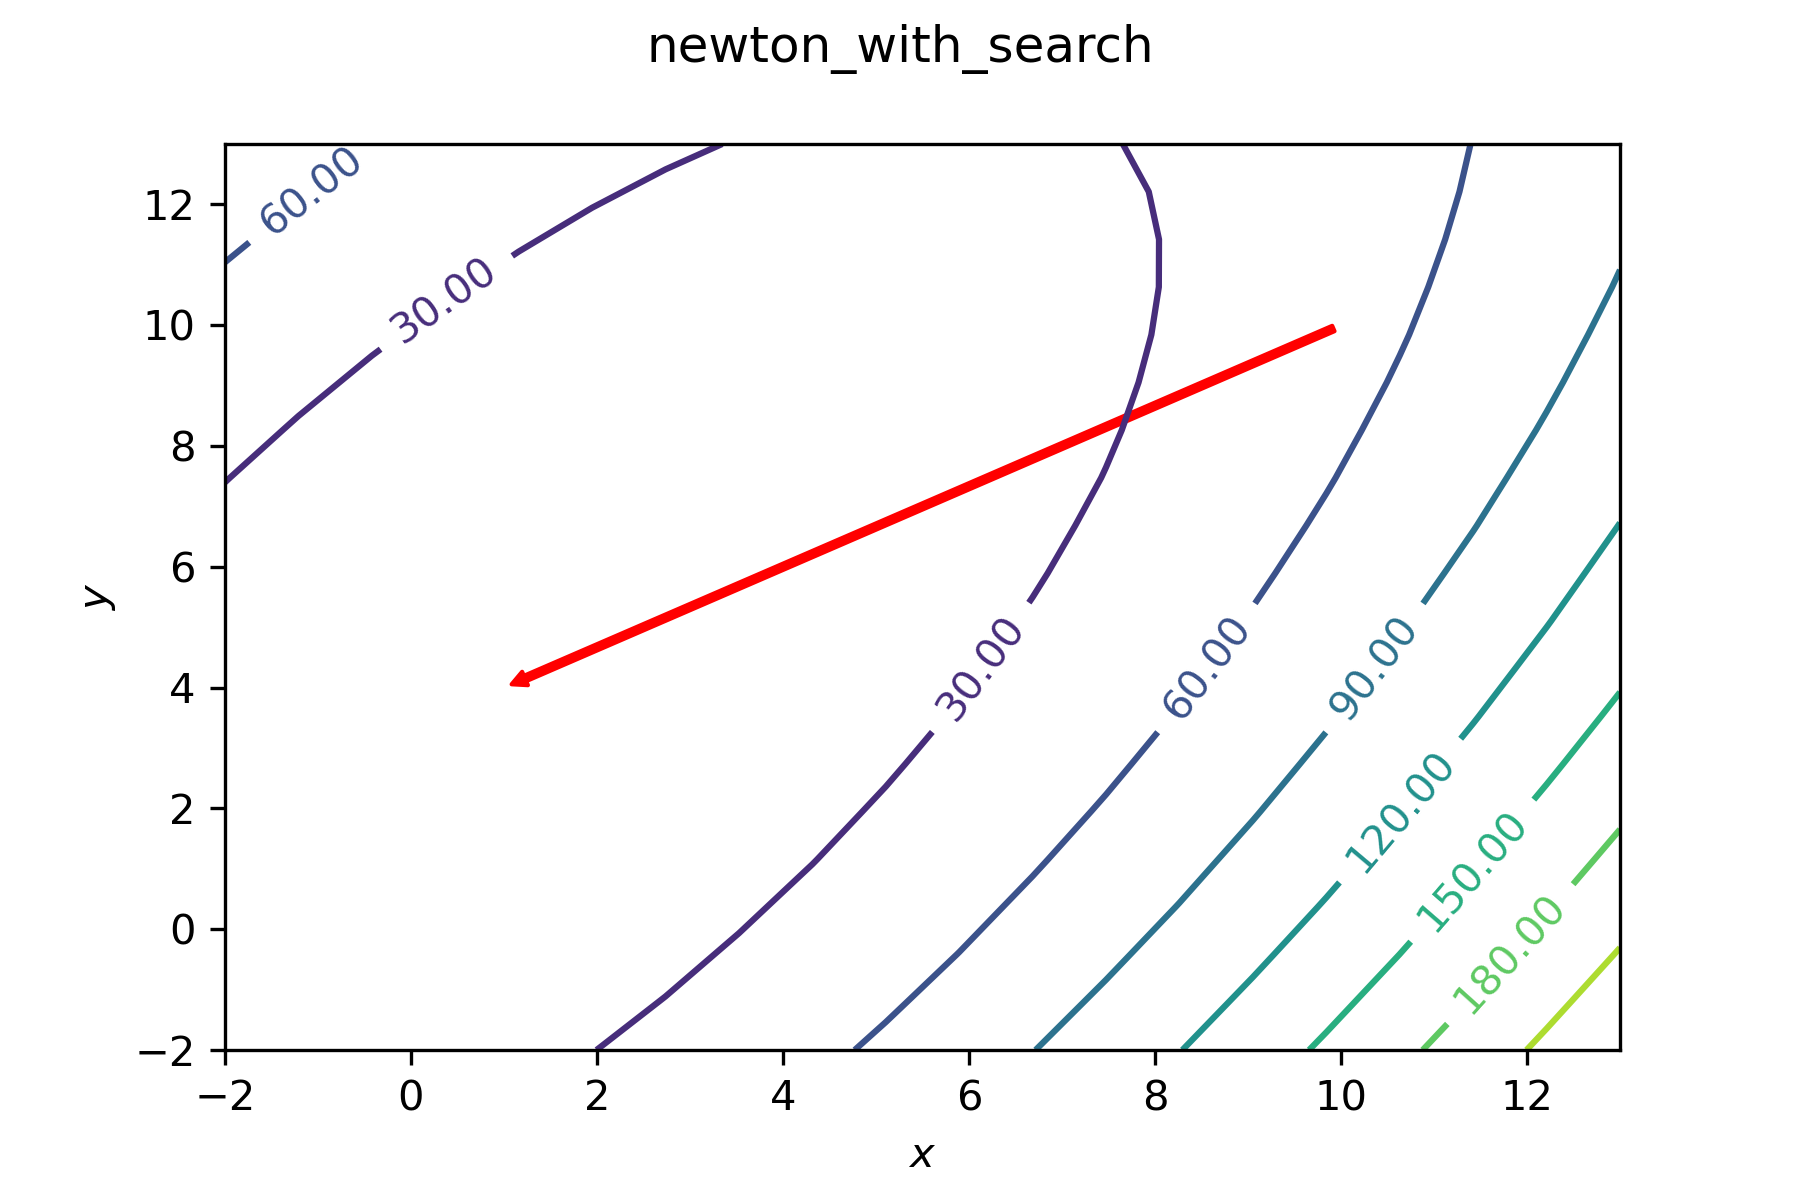
\includegraphics[scale=0.7]{plots/contours_newton_with_search_1.png}
  \end{center}
  \begin{center}
    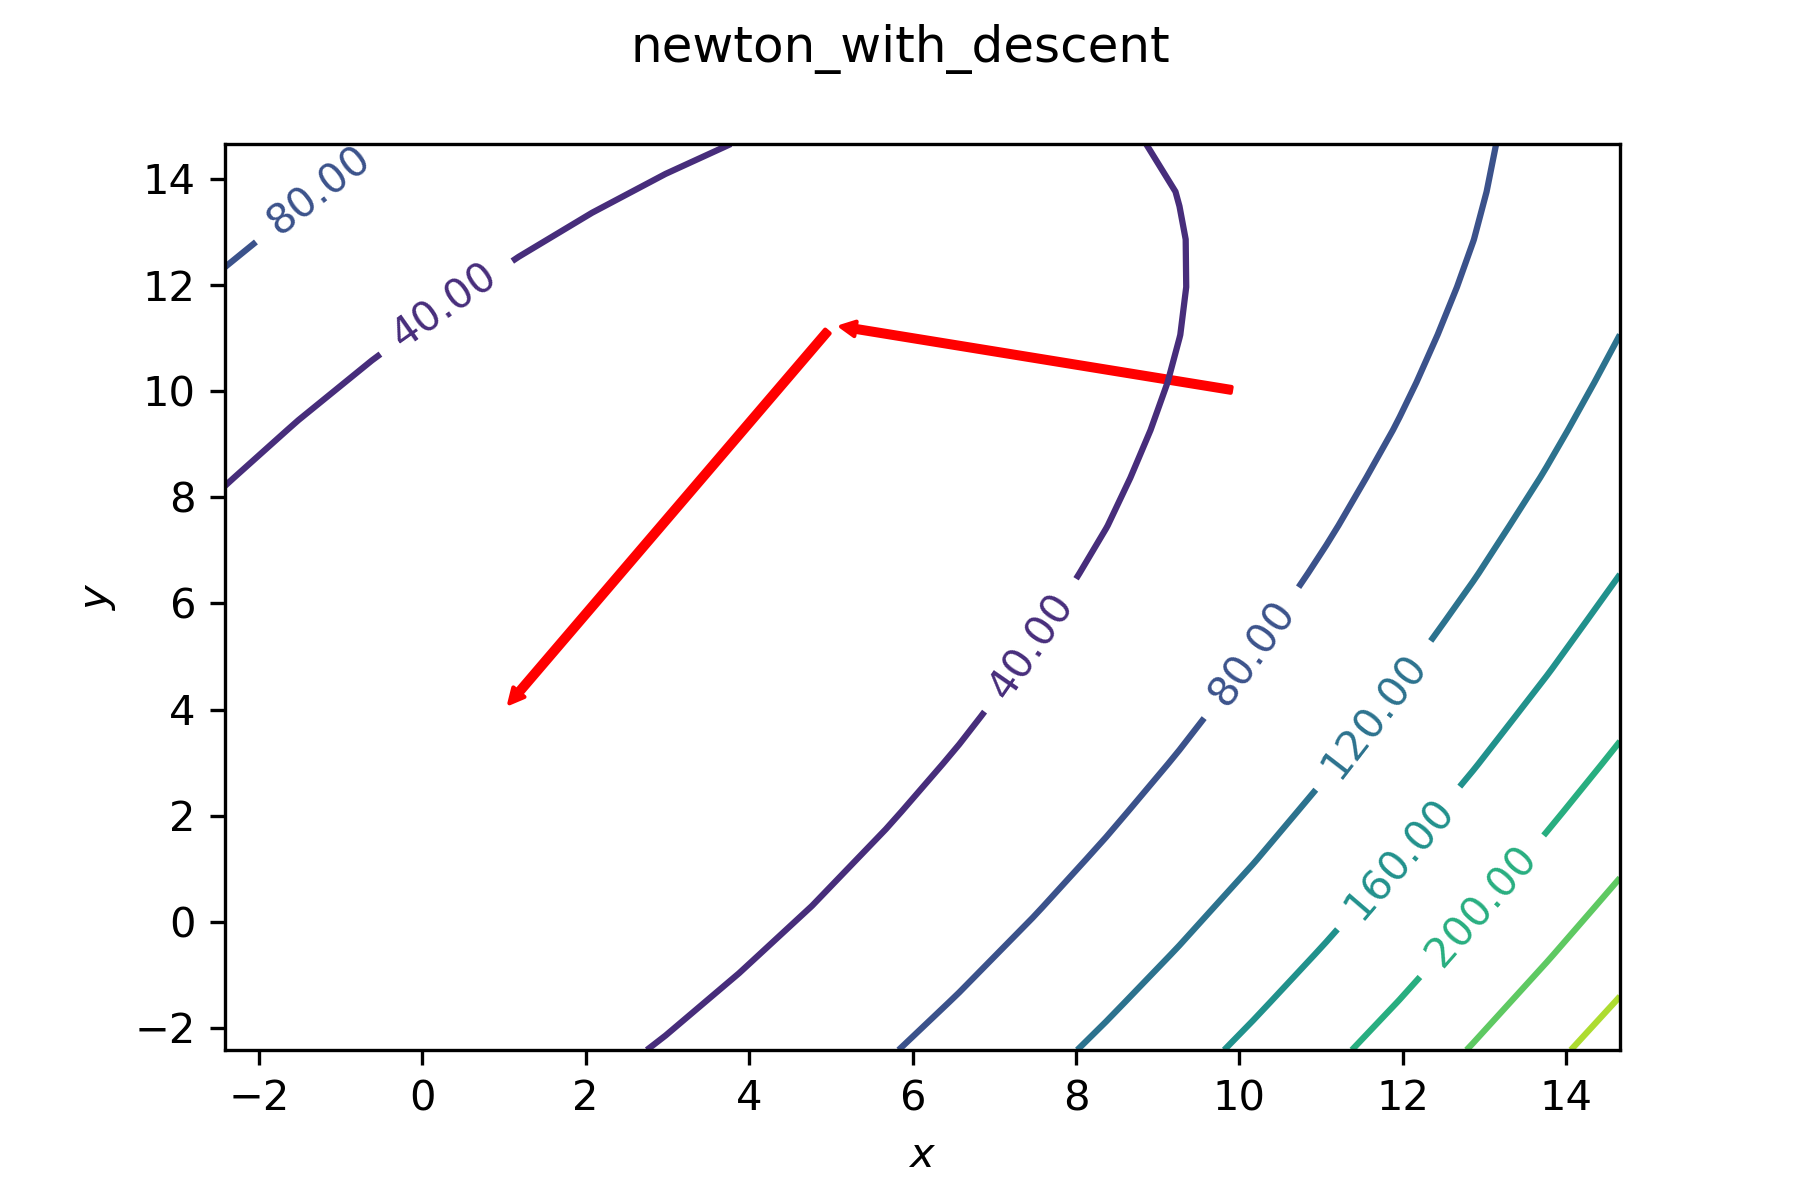
\includegraphics[scale=0.7]{plots/contours_newton_with_descent_1.png}
  \end{center}
Как видно все вариации методы Ньютона находят точку минимума
квадратичной функции за один или два шага. Стоит заметить, что
количество шагов на этой функции не зависит от начального приближения.
\item
  \[ f_2(x, y) = 2 \cdot x^2 + 3 \cdot y^2 + x^2 \cdot y \]
  \[ x_0 = \begin{pmatrix}
    1 & 1
  \end{pmatrix}\]
  \begin{center}
    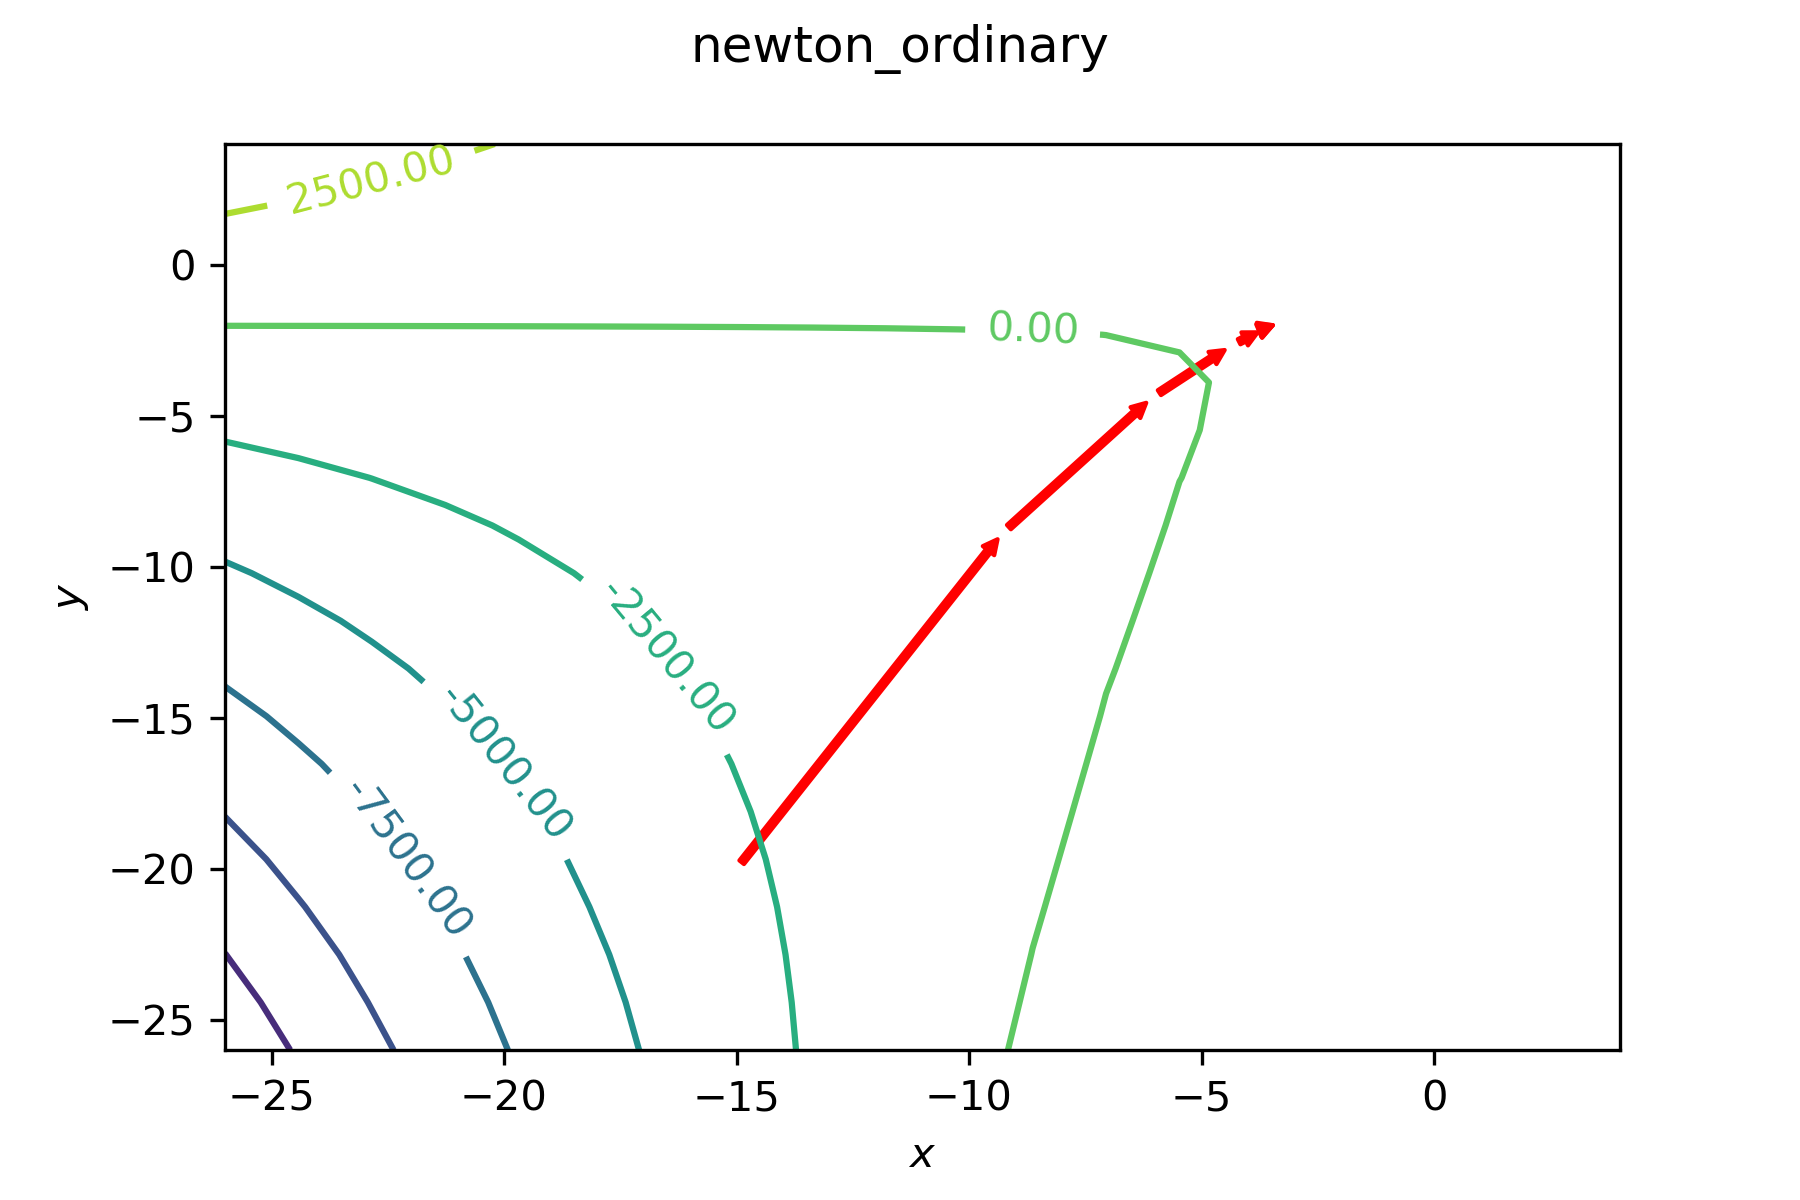
\includegraphics[scale=0.7]{plots/contours_newton_ordinary_2.png}
  \end{center}
  \begin{center}
    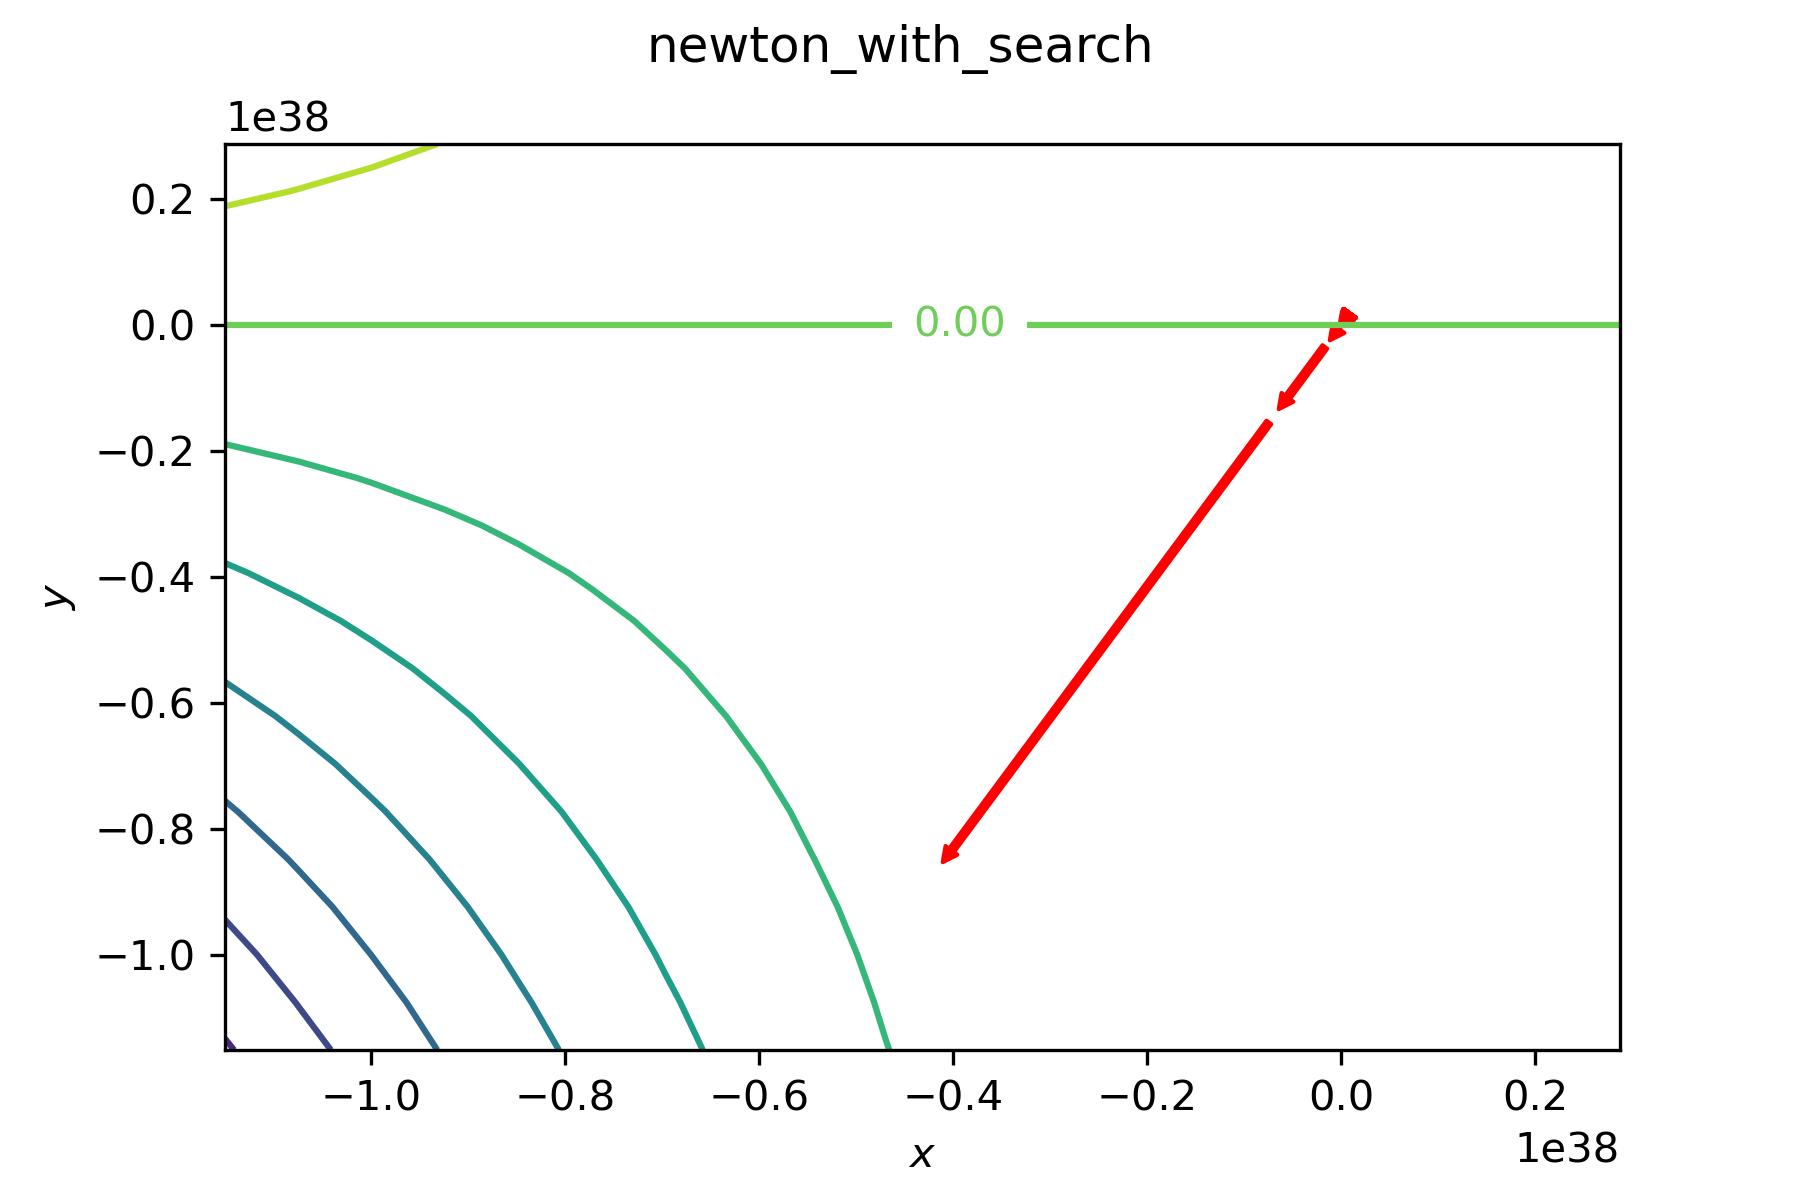
\includegraphics[scale=0.7]{plots/contours_newton_with_search_2.png}
  \end{center}
  \begin{center}
    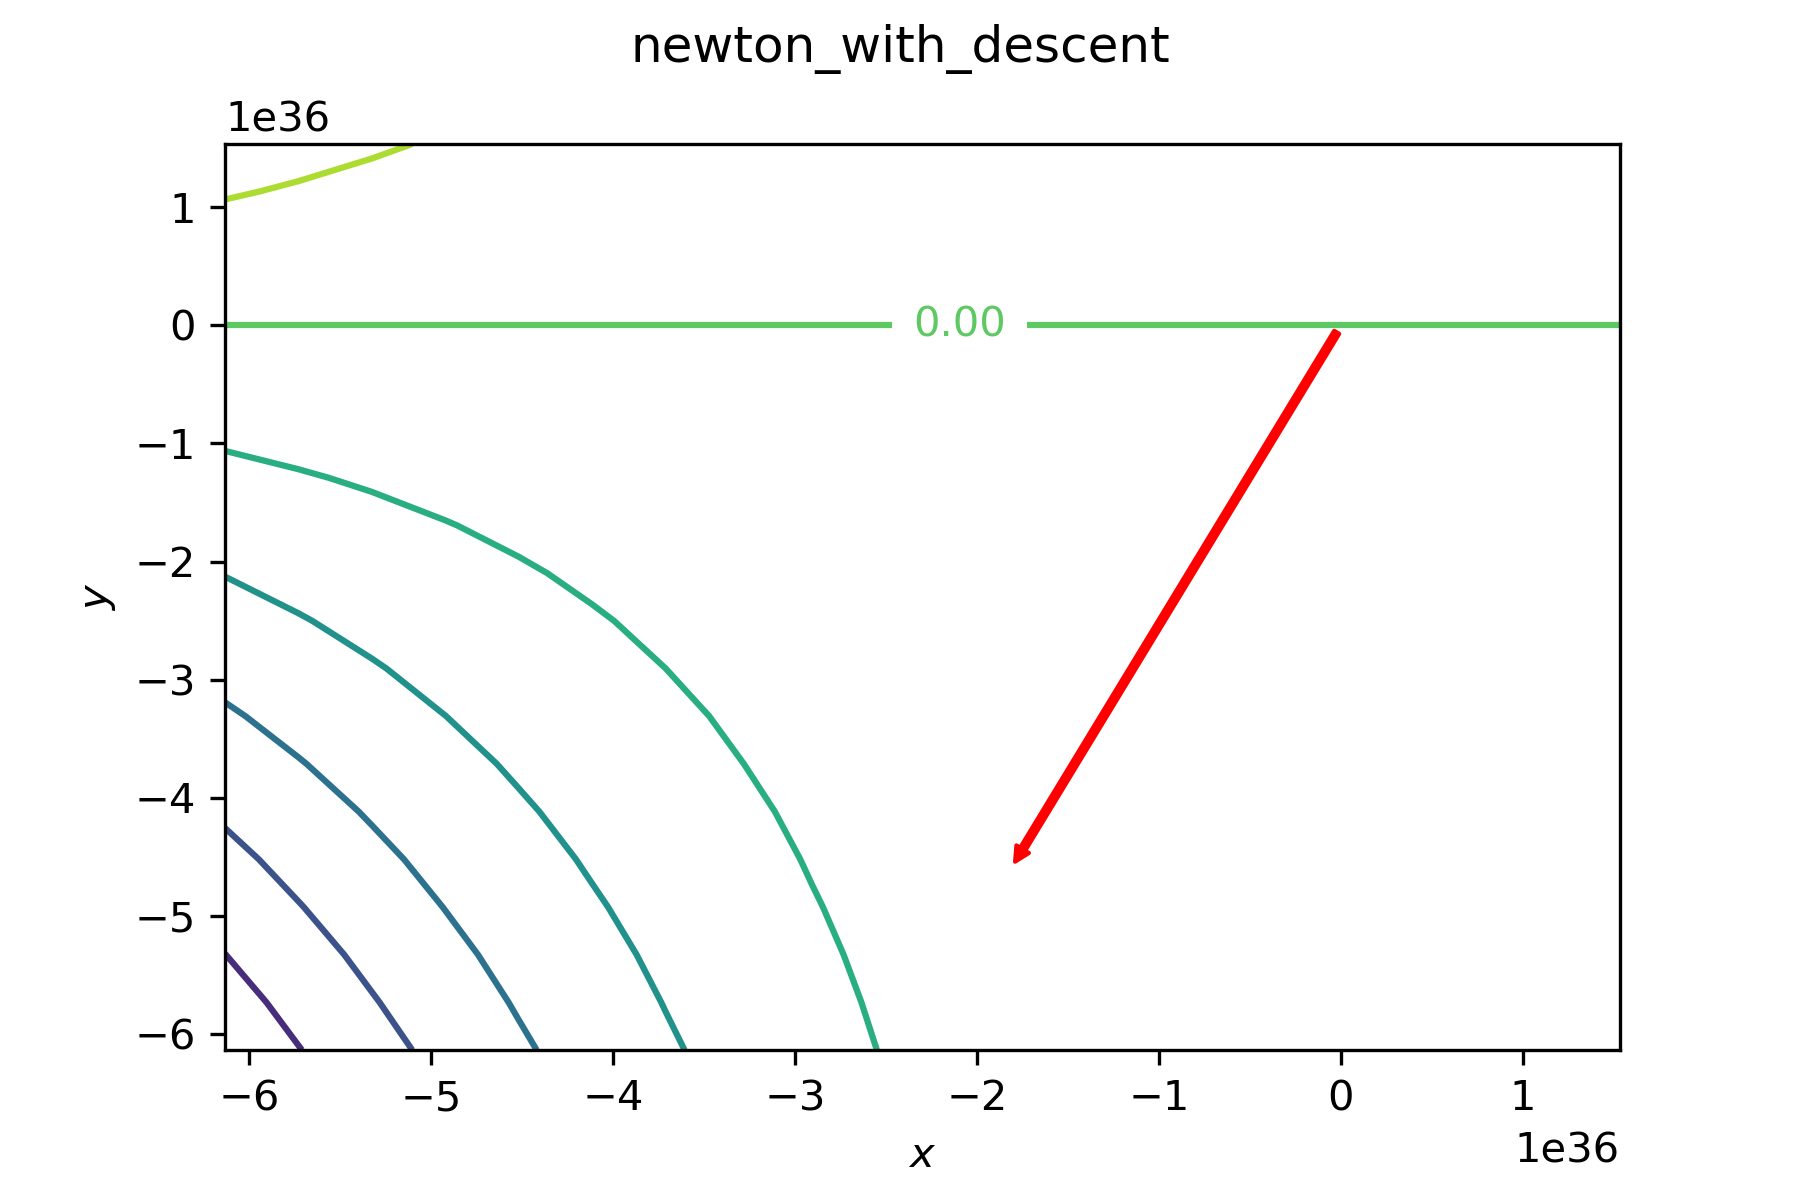
\includegraphics[scale=0.7]{plots/contours_newton_with_descent_2.png}
  \end{center}
\begin{center}
  \begin{longtable}{l|cc}
    Метод & Итерация & \(\alpha\) \\
    \hline
    Метод Ньютона с одномерным поиском & 1 & 1 \\
    & 2 & \(-9.99886\)
    \hline
    Метод Ньютона с направлением спуска & 1 & \(0.4\) \\
    & 2 & \(1\) \\
    & 3 & \(-9.99886\)
  \end{longtable}
\end{center}
  На второй функции ситуация немного другая: обычный метод ньютона
  делает маленький шаг и находит локальный минимум за небольшое
  количество шагов, другие две модификации делают достаточно большой
  шаг и попадают соответственно в точки где градиент функции равен \(0\),
  либо функция бесконечно убывает. Из-за этого решение \(p\) не
  существует. Это выглядит примерно так:
  \begin{center}
    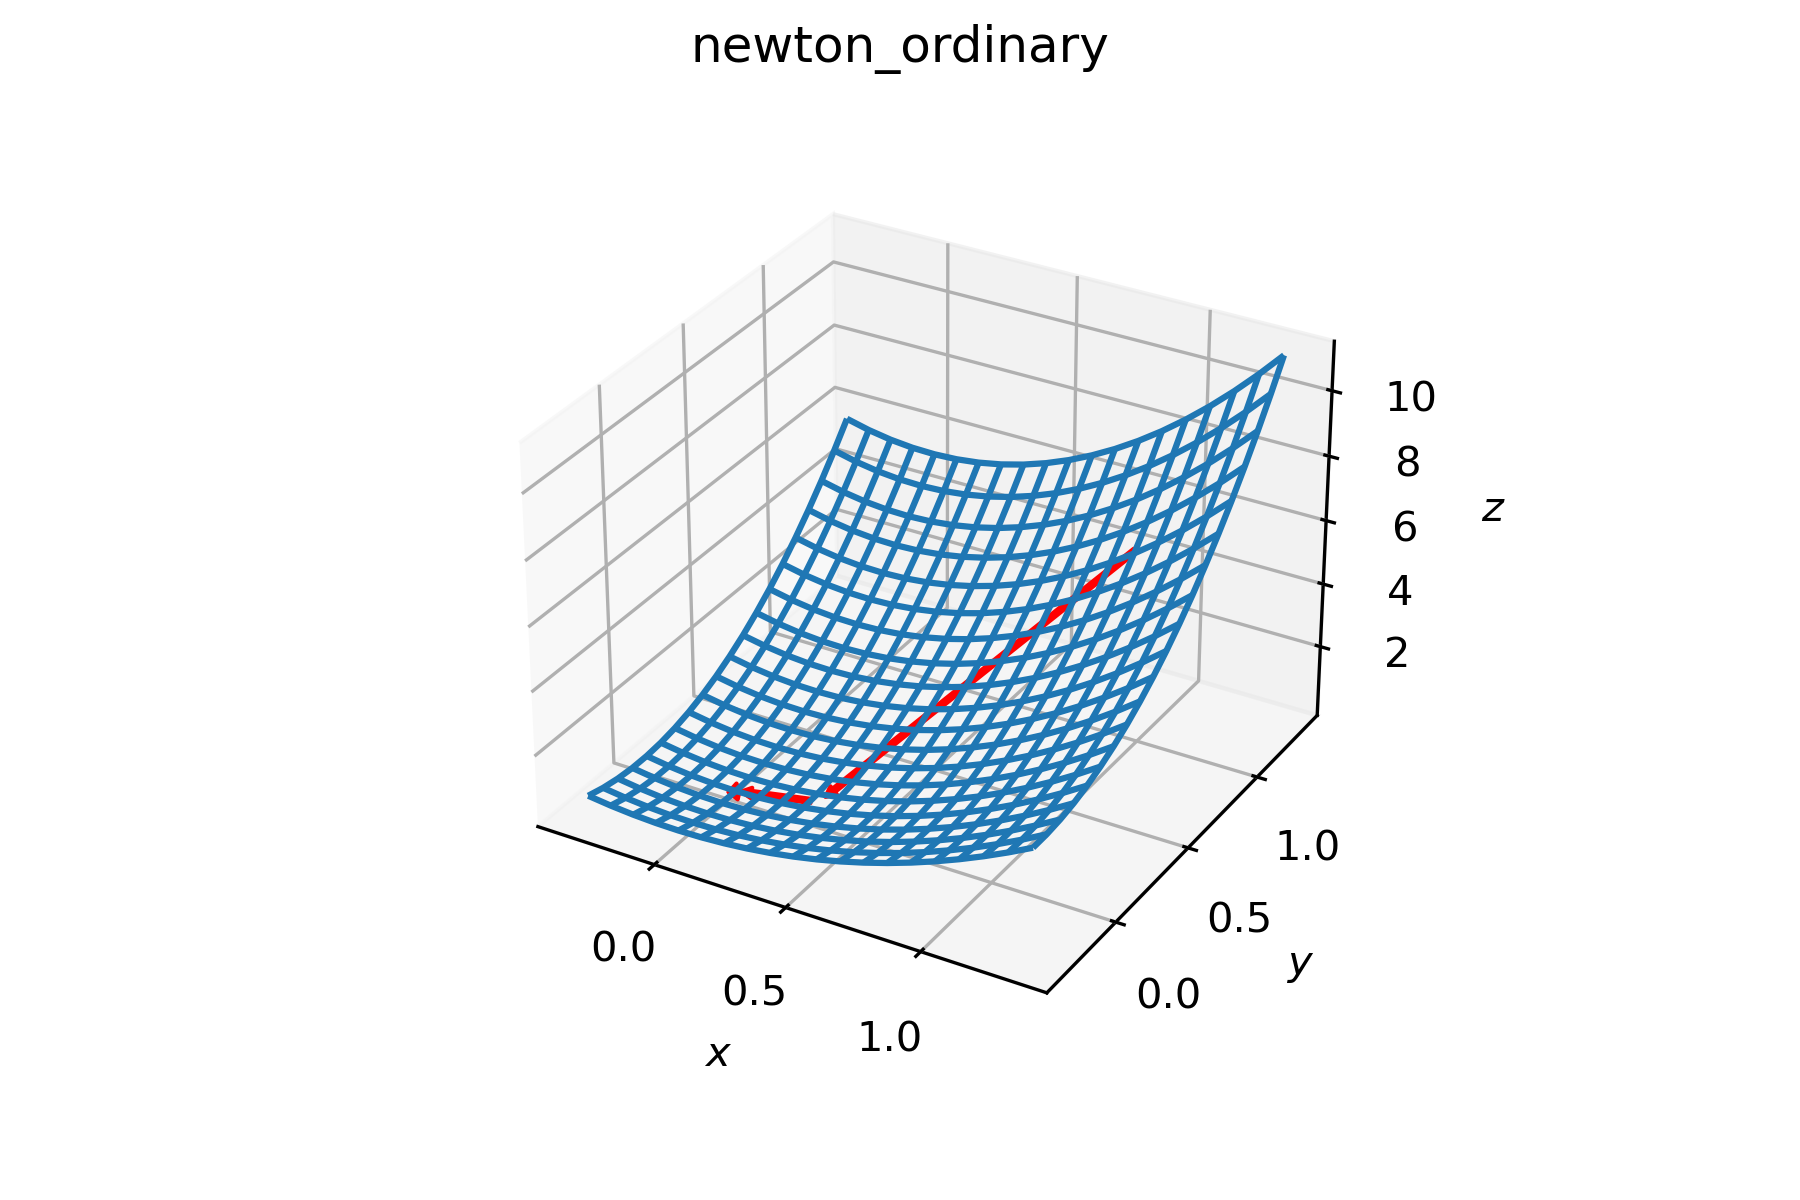
\includegraphics[scale=0.7]{plots/3D_newton_ordinary_2.png}
  \end{center}
  \begin{center}
    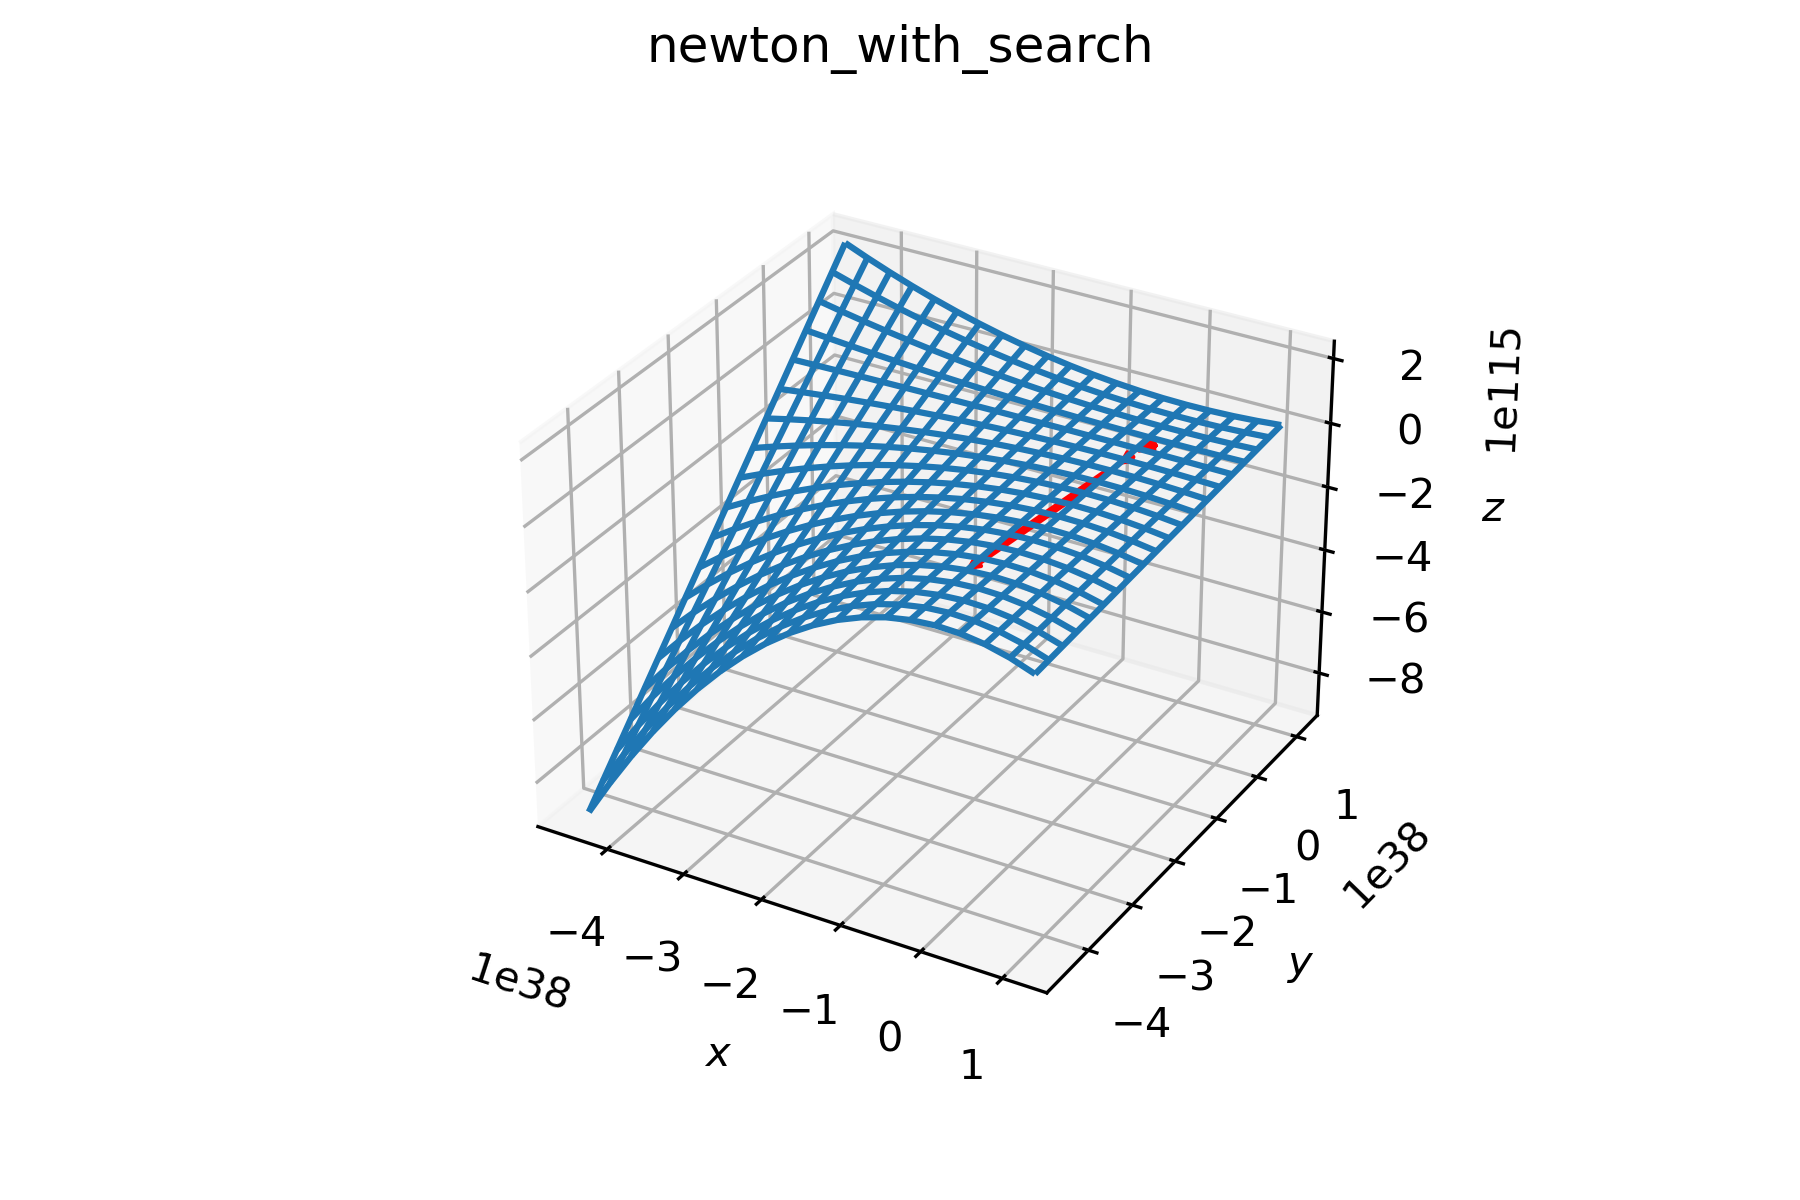
\includegraphics[scale=0.7]{plots/3D_newton_with_search_2.png}
  \end{center}
  \begin{center}
    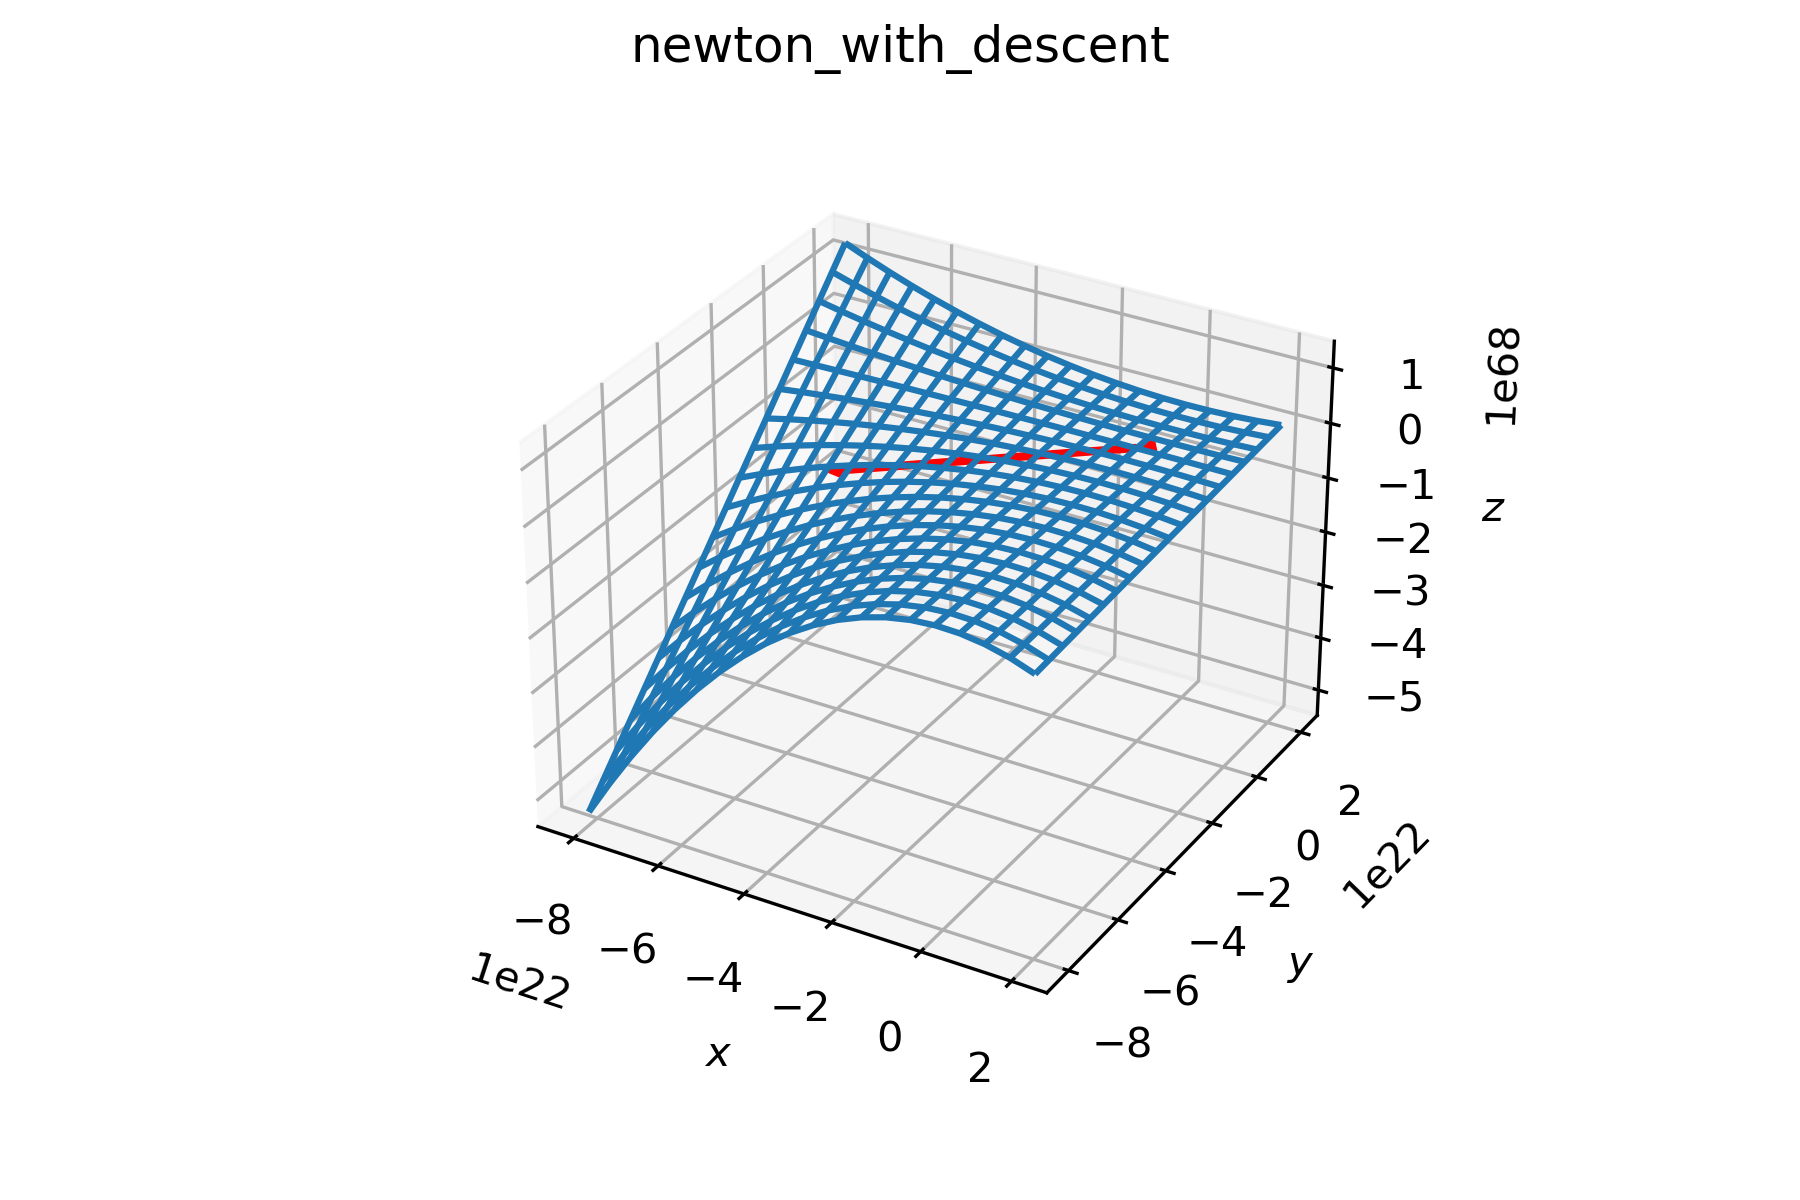
\includegraphics[scale=0.7]{plots/3D_newton_with_descent_2.png}
  \end{center}
\end{enumerate}
\begin{center}
  \begin{longtable}{l|cc}
    Метод & Количество итераций на \(f_1\) & Количество итераций на \(f_2\) \\
    \hline
    Метод Ньютона & 2 & 4 \\
    \hline
    Метод Ньютона с одномерным поиском & 2 & 50 \\
    \hline
    Метод Ньютона с направлением спуска & 3 & 5 \\
  \end{longtable}
\end{center}
На квадратичной функции все методы совершают примерно равное малое
количество итераций. На произвольной функций некоторые методы, в нашем
случае метод с одномерным поиском, могут застревать в точках, похожих
на локальный минимум, но затем совершать достаточный шаг для
преодоления места возрастания функции.


Таблица с количеством итераций при различных начальных приближениях:
\[ x_1 = \begin{pmatrix}
  1, 1
\end{pmatrix} \quad x_2 = \begin{pmatrix}
  10, 10
\end{pmatrix} \quad x_3 = \begin{pmatrix}
  -15, -20
\end{pmatrix}\]
\begin{center}
  \begin{longtable}{l|l|l|l}
    Начальное приближение & Обычный & С одномерным поиском & С направлением спуска \\
    \hline
    \(x_1\) & 5 & 50 & 5 \\
    \hline
    \(x_2\) & 7 & 49 & 5 \\
    \hline
    \(x_3\) & 8 & 48 & 5 \\
  \end{longtable}
\end{center}
Видно, что метод Ньютона с направлением спуска совершает на порядок
больше шагов, в отличие от двух других методов. Стоит также заметить
что модификации метода Ньютона на всех начальных приближения уходят в
те точки, где функция бесконечно убывает, а обычный сходится в
локальный минимум.
\subsection{Исследование на заданных функциях}
\[ f_1(x, y) = x^2 + y^2  - 1.2xy \quad x_0 = \begin{pmatrix}
  4 & 1
\end{pmatrix}\]
\begin{center}
  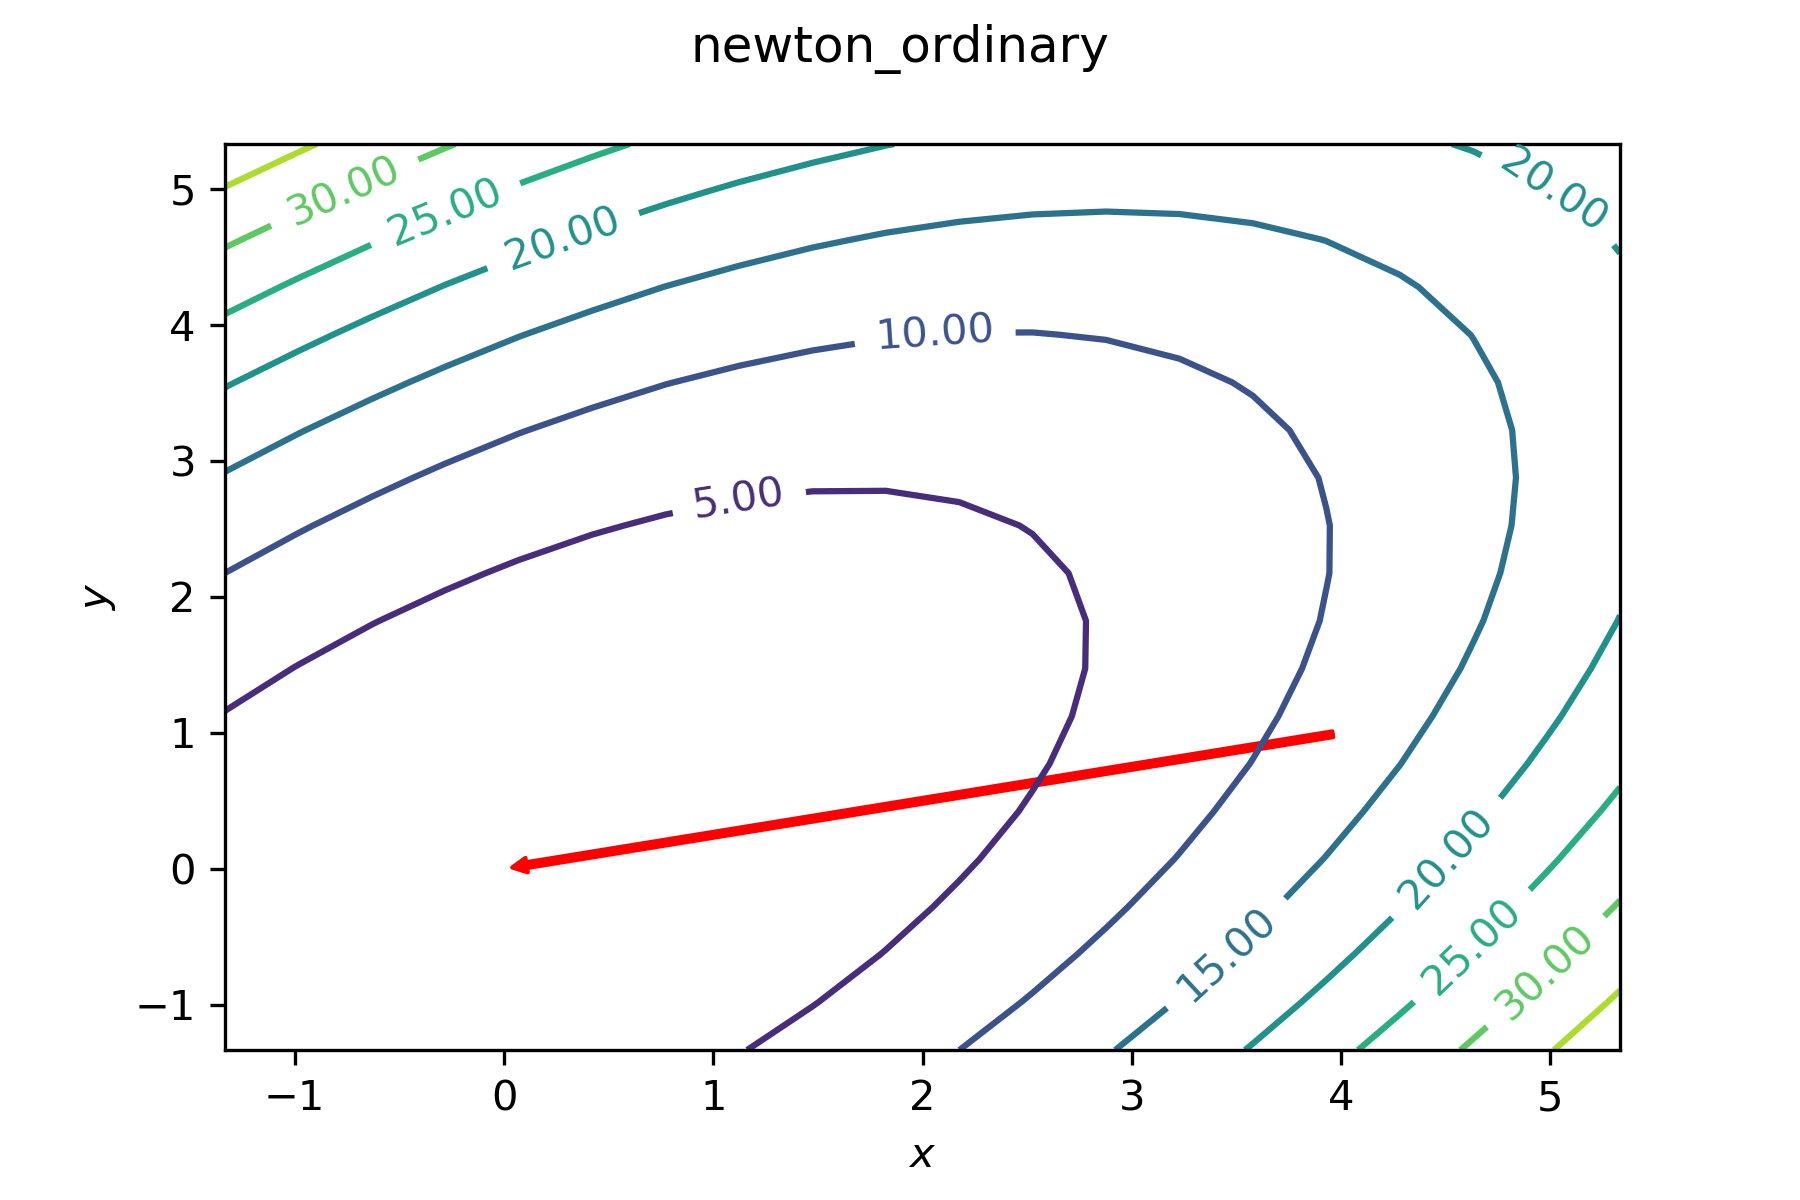
\includegraphics[scale=0.7]{plots/contours_newton_ordinary_4.png}
\end{center}
\begin{center}
  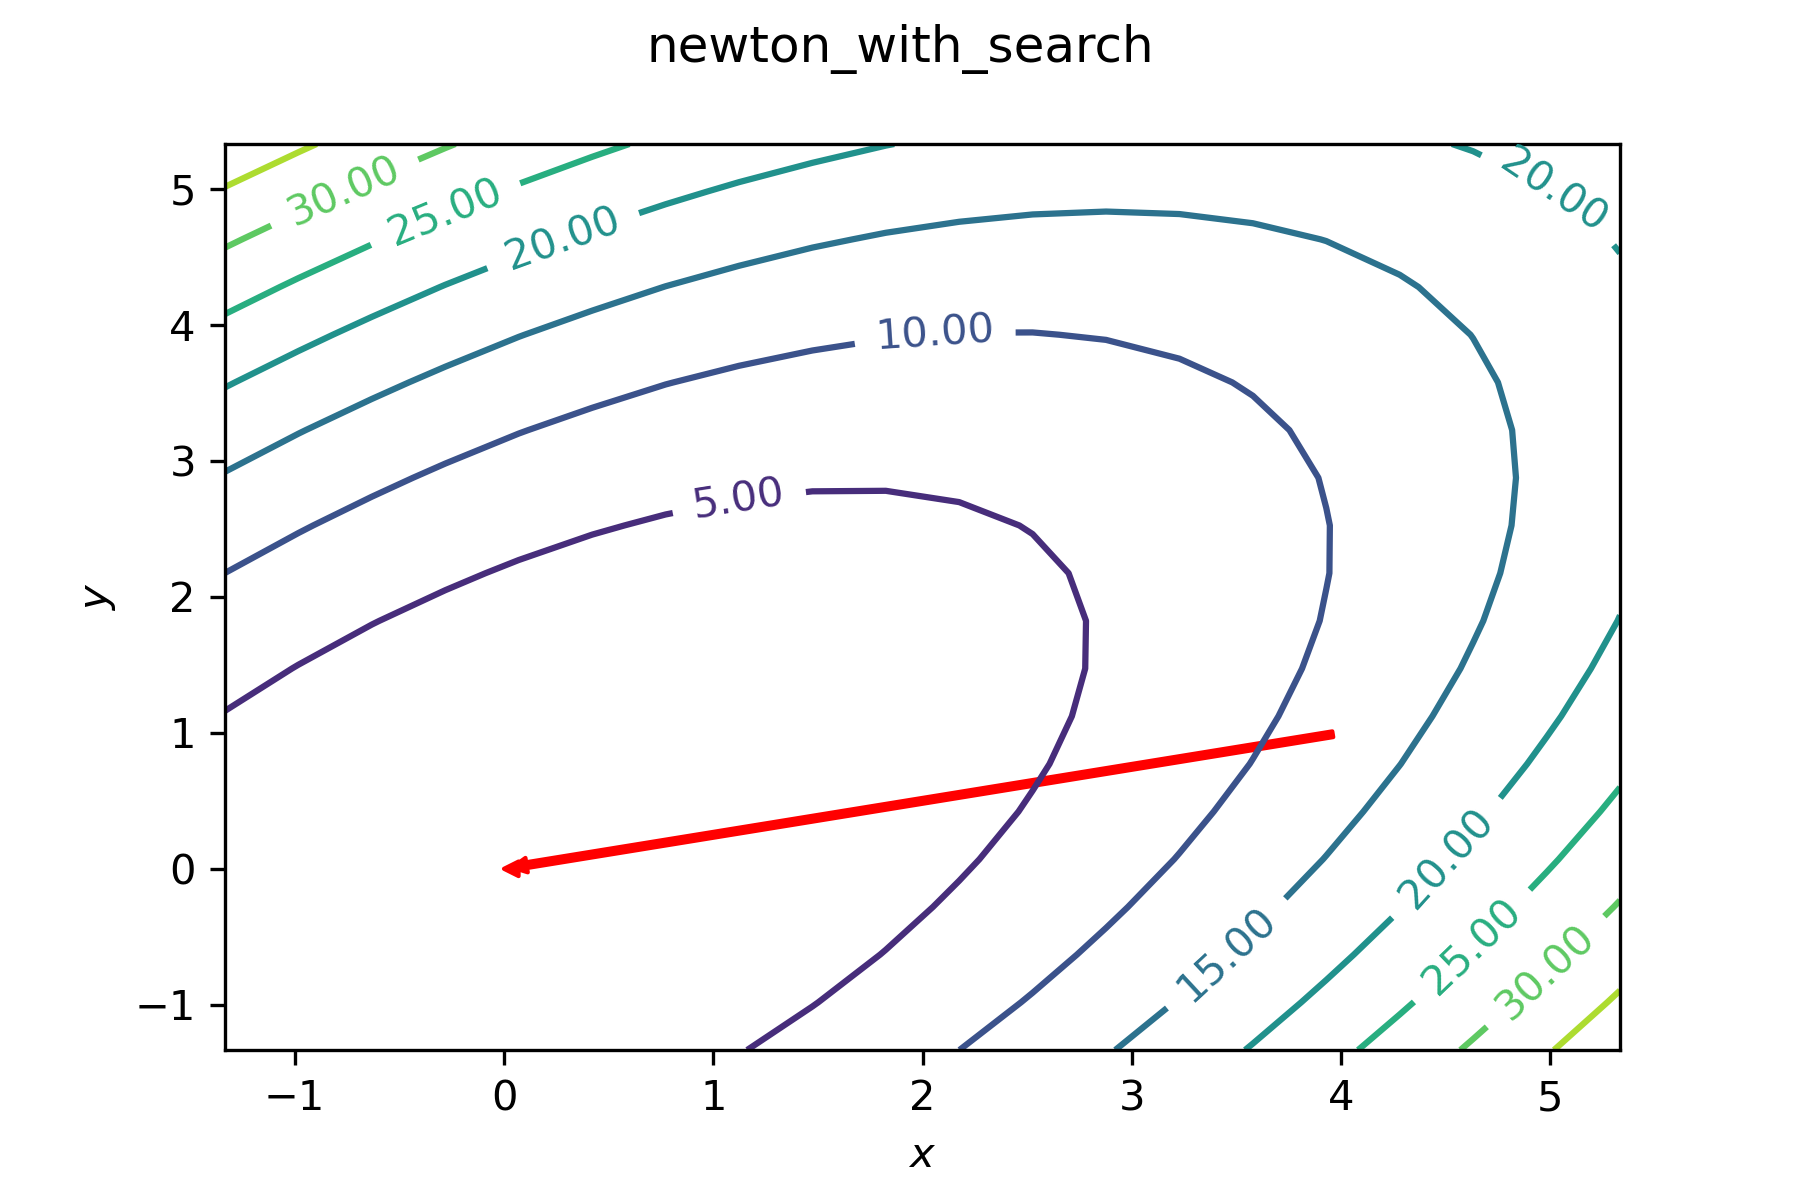
\includegraphics[scale=0.7]{plots/contours_newton_with_search_4.png}
\end{center}
\begin{center}
  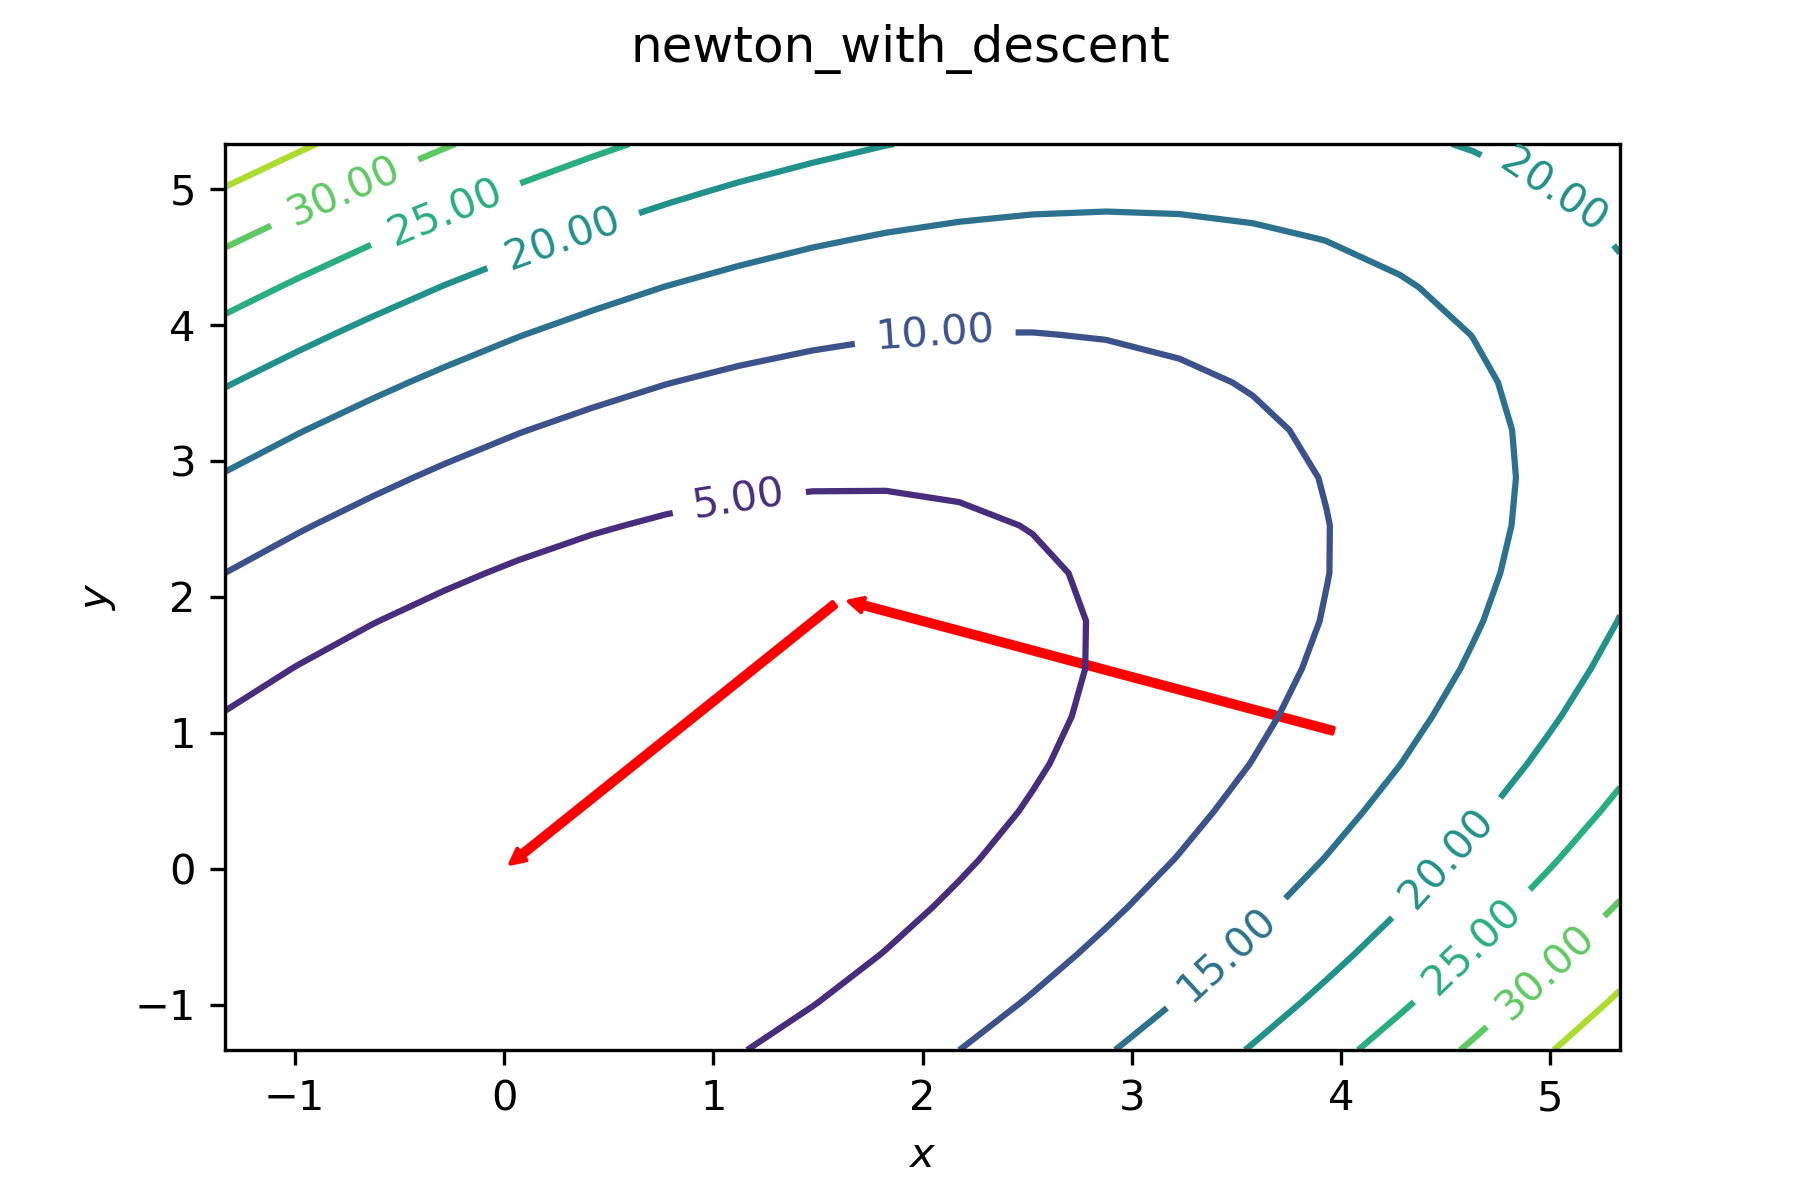
\includegraphics[scale=0.7]{plots/contours_newton_with_descent_4.png}
\end{center}
\[ f_2(x, y) = 100(y - x^2)^2 + (1 - x)^2 \quad x_0 = \begin{pmatrix}
  -1.2 & 1
\end{pmatrix}\]
\begin{center}
  \begin{longtable}{l|cc}
    Метод & Количество итераций \\
    \hline
    Метод Ньютона & 3 \\
    \hline
    Метод Ньютона с одномерным поиском & 3 \\
    \hline
    Метод Ньютона с направлением спуска &  4 \\
  \end{longtable}
\end{center}
Все методы сходятся к точке \(x^*: f(x^*) \approx 0\)
\begin{center}
  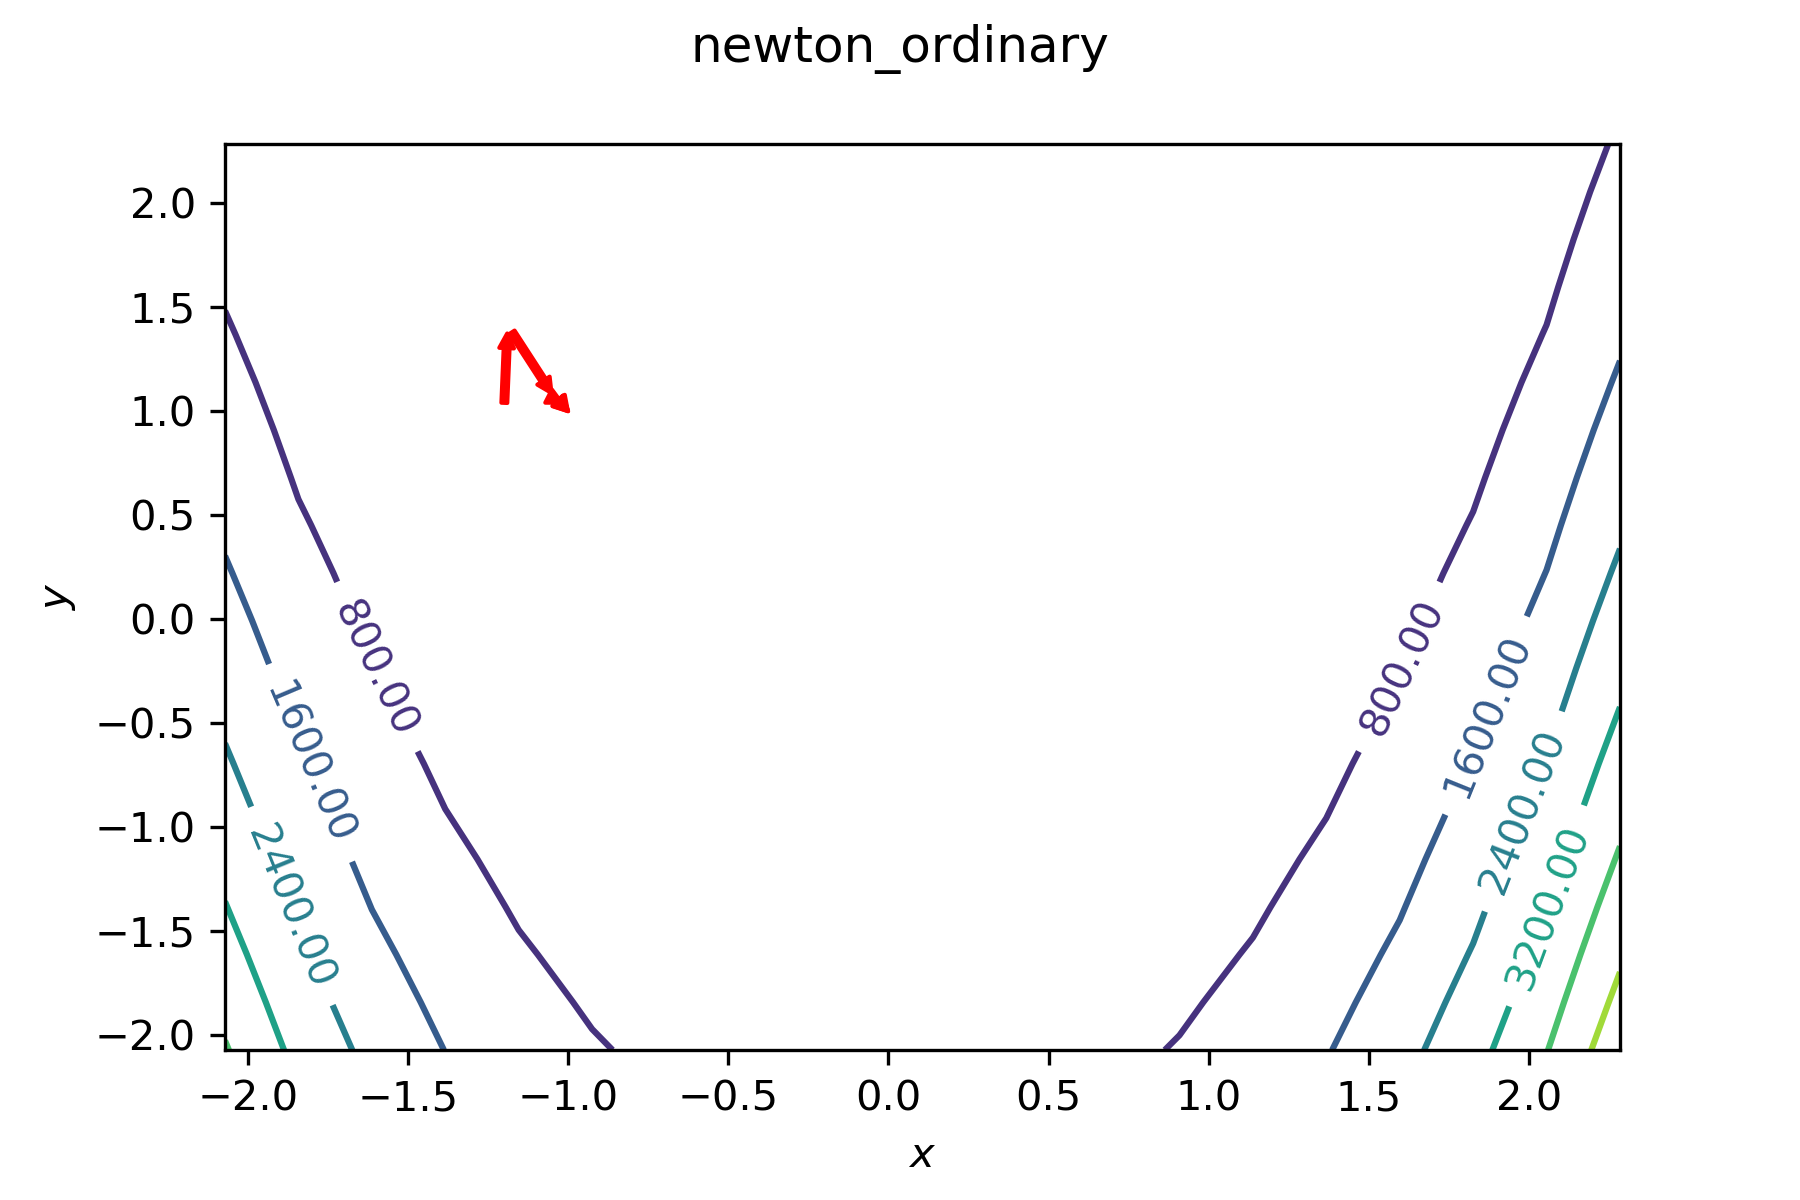
\includegraphics[scale=0.7]{plots/contours_newton_ordinary_5.png}
\end{center}
\begin{center}
  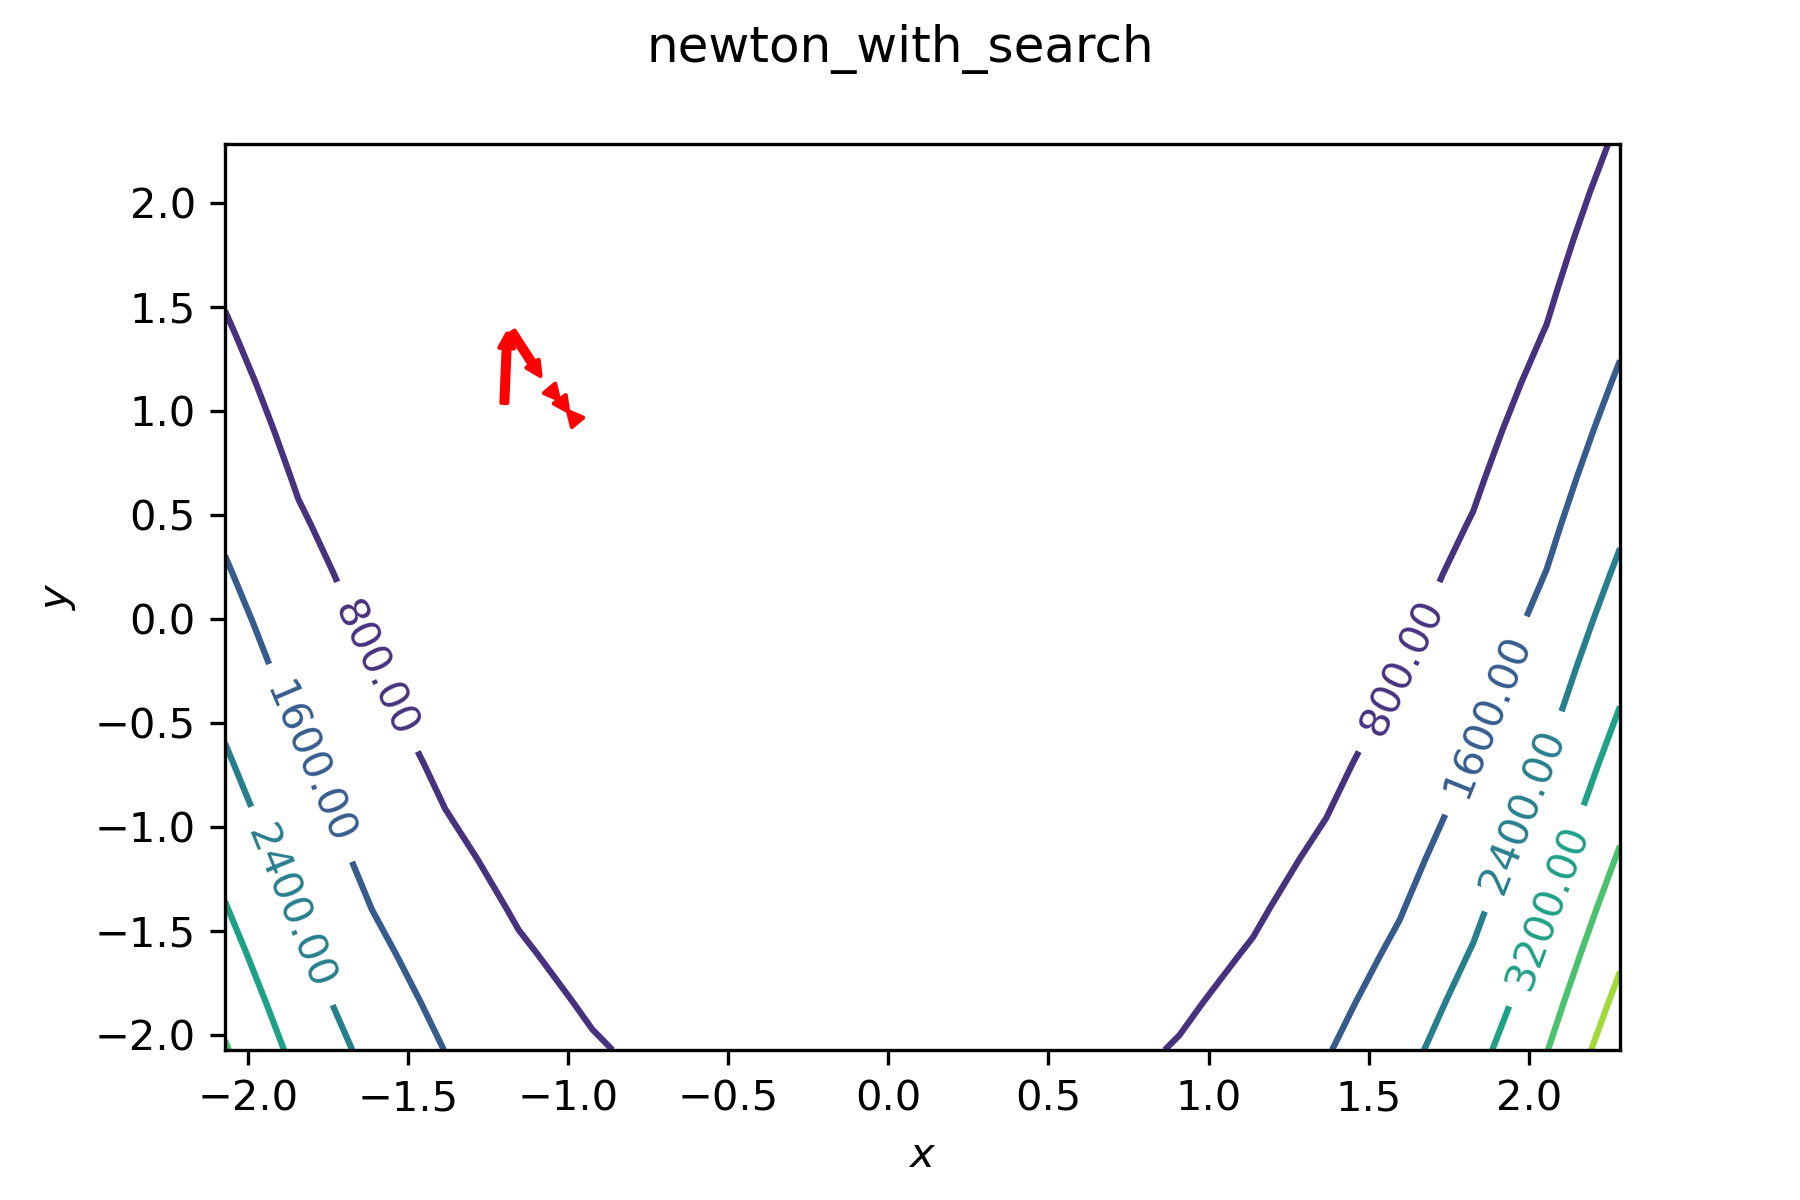
\includegraphics[scale=0.7]{plots/contours_newton_with_search_5.png}
\end{center}
\begin{center}
  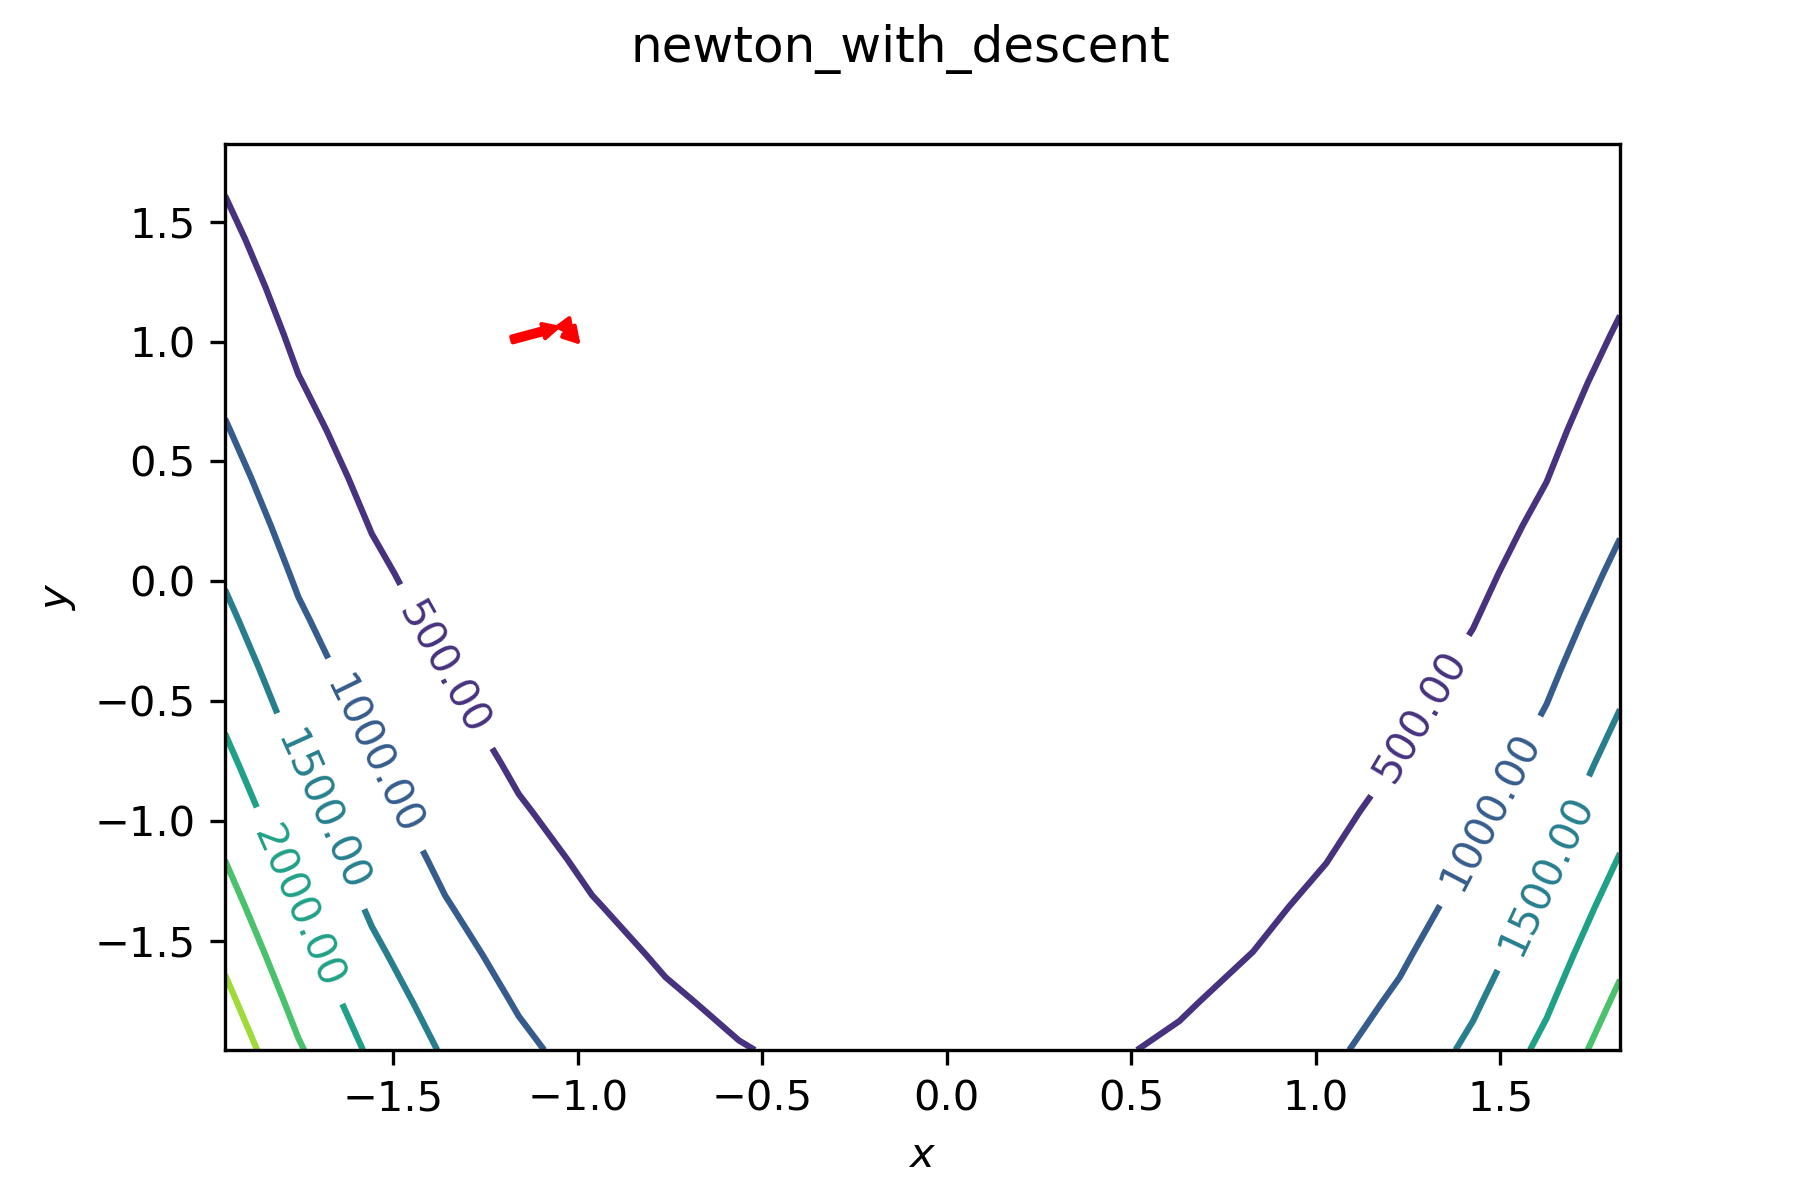
\includegraphics[scale=0.7]{plots/contours_newton_with_descent_5.png}
\end{center}
\begin{center}
  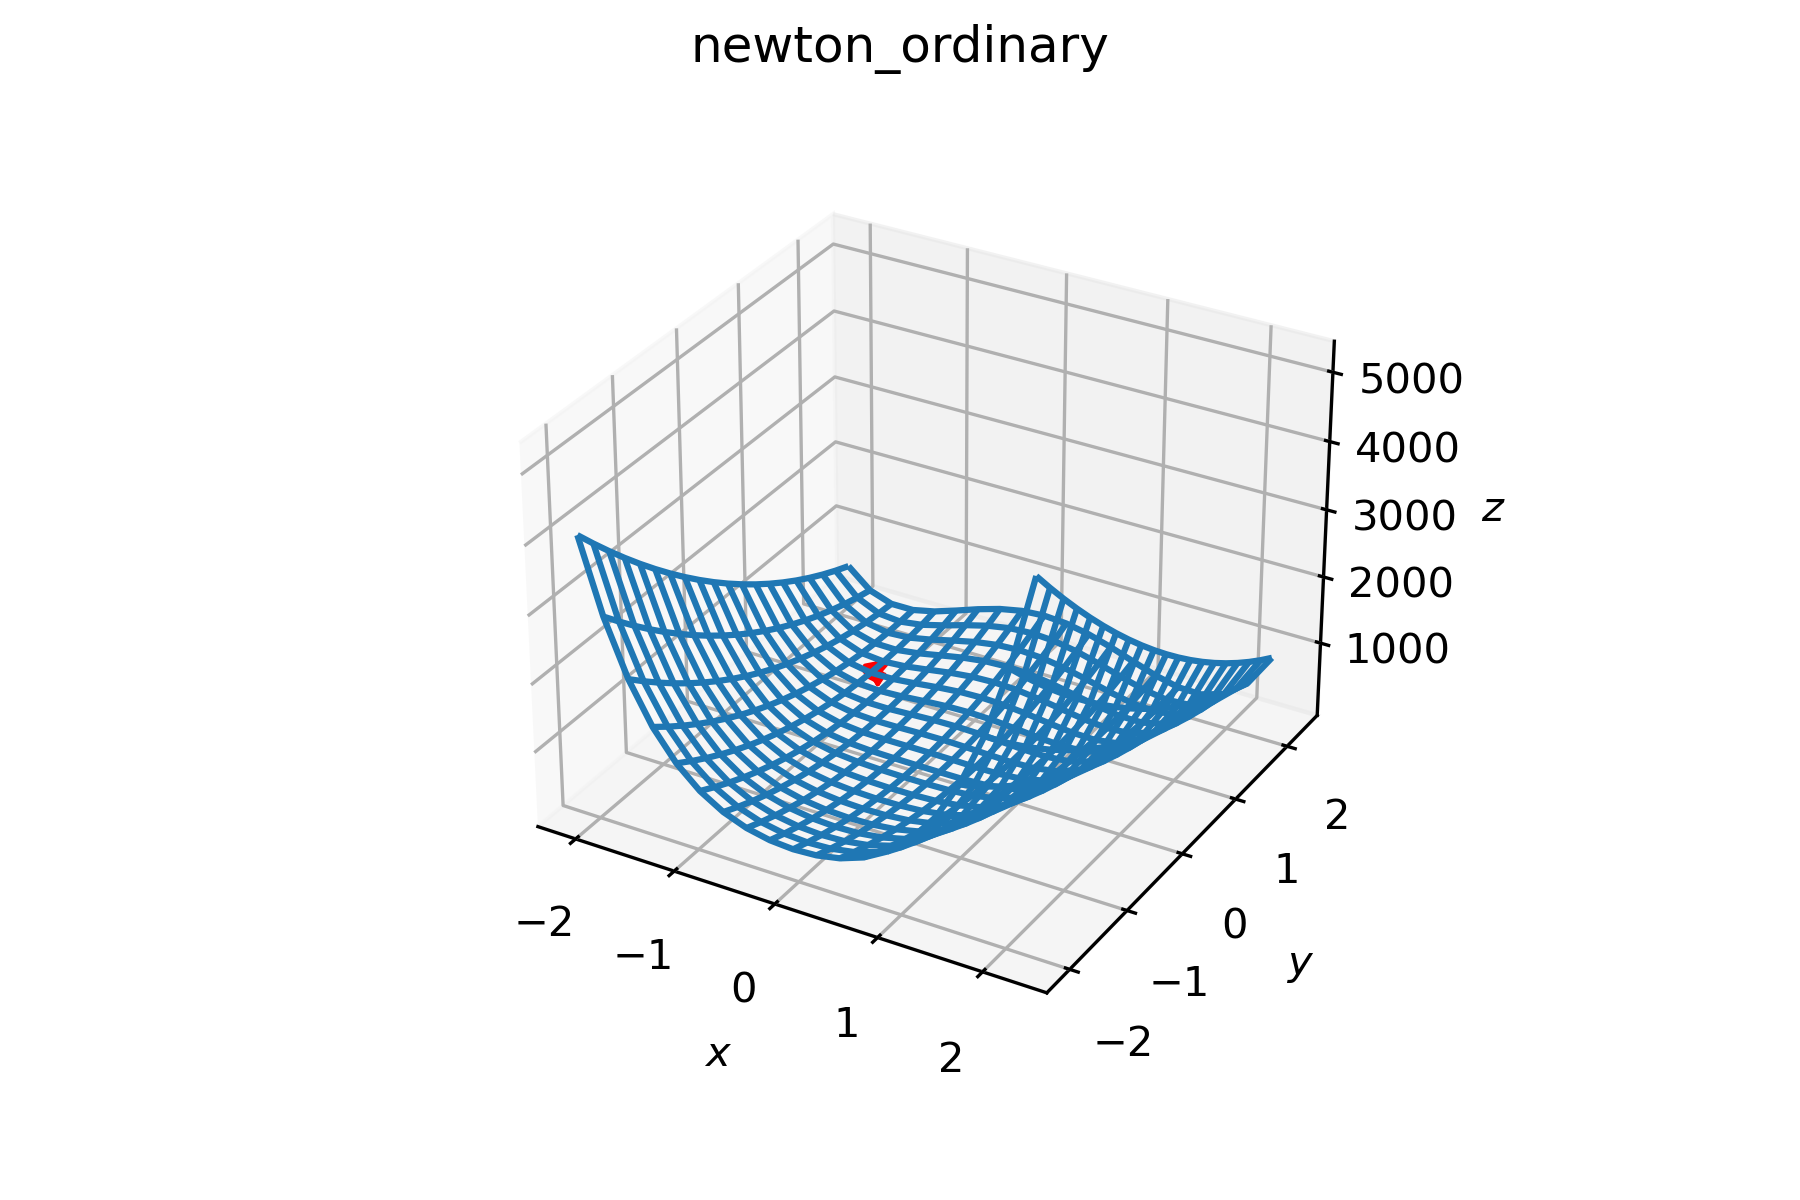
\includegraphics[scale=0.7]{plots/3D_newton_ordinary_5.png}
\end{center}
\begin{center}
  \begin{longtable}{l|cc}
    Метод & Количество итераций \\
    \hline
    Метод Ньютона & 7 \\
    \hline
    Метод Ньютона с одномерным поиском & 7 \\
    \hline
    Метод Ньютона с направлением спуска &  6 \\
  \end{longtable}
\end{center}
Все методы сходятся к точке \(x^*: f(x^*) = 0\).

Все методы показывают себя примерно одинаково, но в некоторых случаях
метод с одномерным поиском совершает намного больше итераций в отличие
от остальных. В целом можно сказать, что метод с направлением спуска
работает лучше, так как совершает меньшее число итераций на
большинстве функций и начальных приближениях.
\subsection{Квазиньютоновские методы}
\subsubsection{Схема работы}
Общая схема работы похожа на схему методов Ньютона, однако данные
методы отличаются от методов Ньютона тем что не требуют решать СЛАУ на
каждой итерации. Вместо этого выбирается такая последовательность
матриц \(G_k\), что \(G_k \to H^{-1}\)
\subsubsection{Исследование на функциях}
\[ f_1(x) = 100(x_2 - x_1^2)^2 + (1 - x_1)^2  \quad x_0 = \begin{pmatrix}
  10 & 0
\end{pmatrix}\]
\begin{center}
  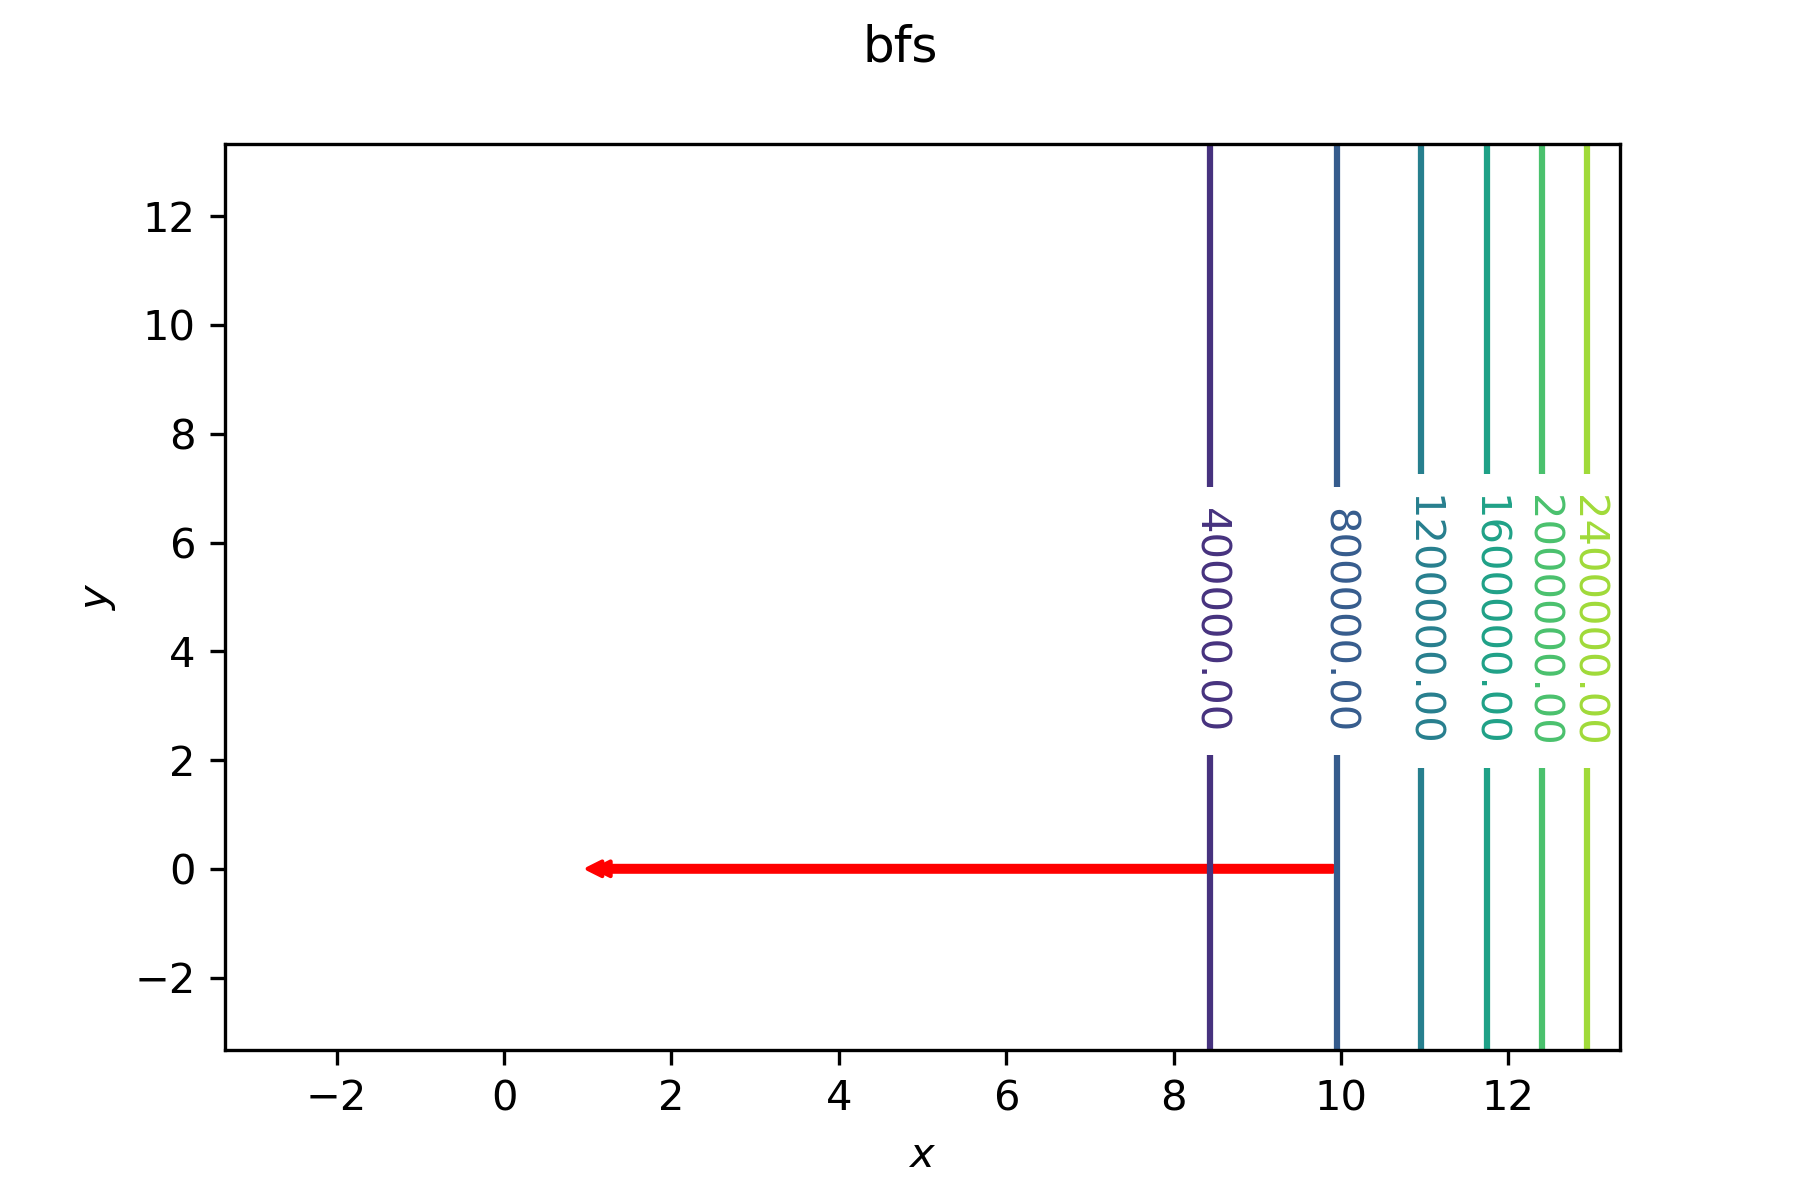
\includegraphics[scale=0.7]{plots/contours_bfs_6.png}
\end{center}
\begin{center}
  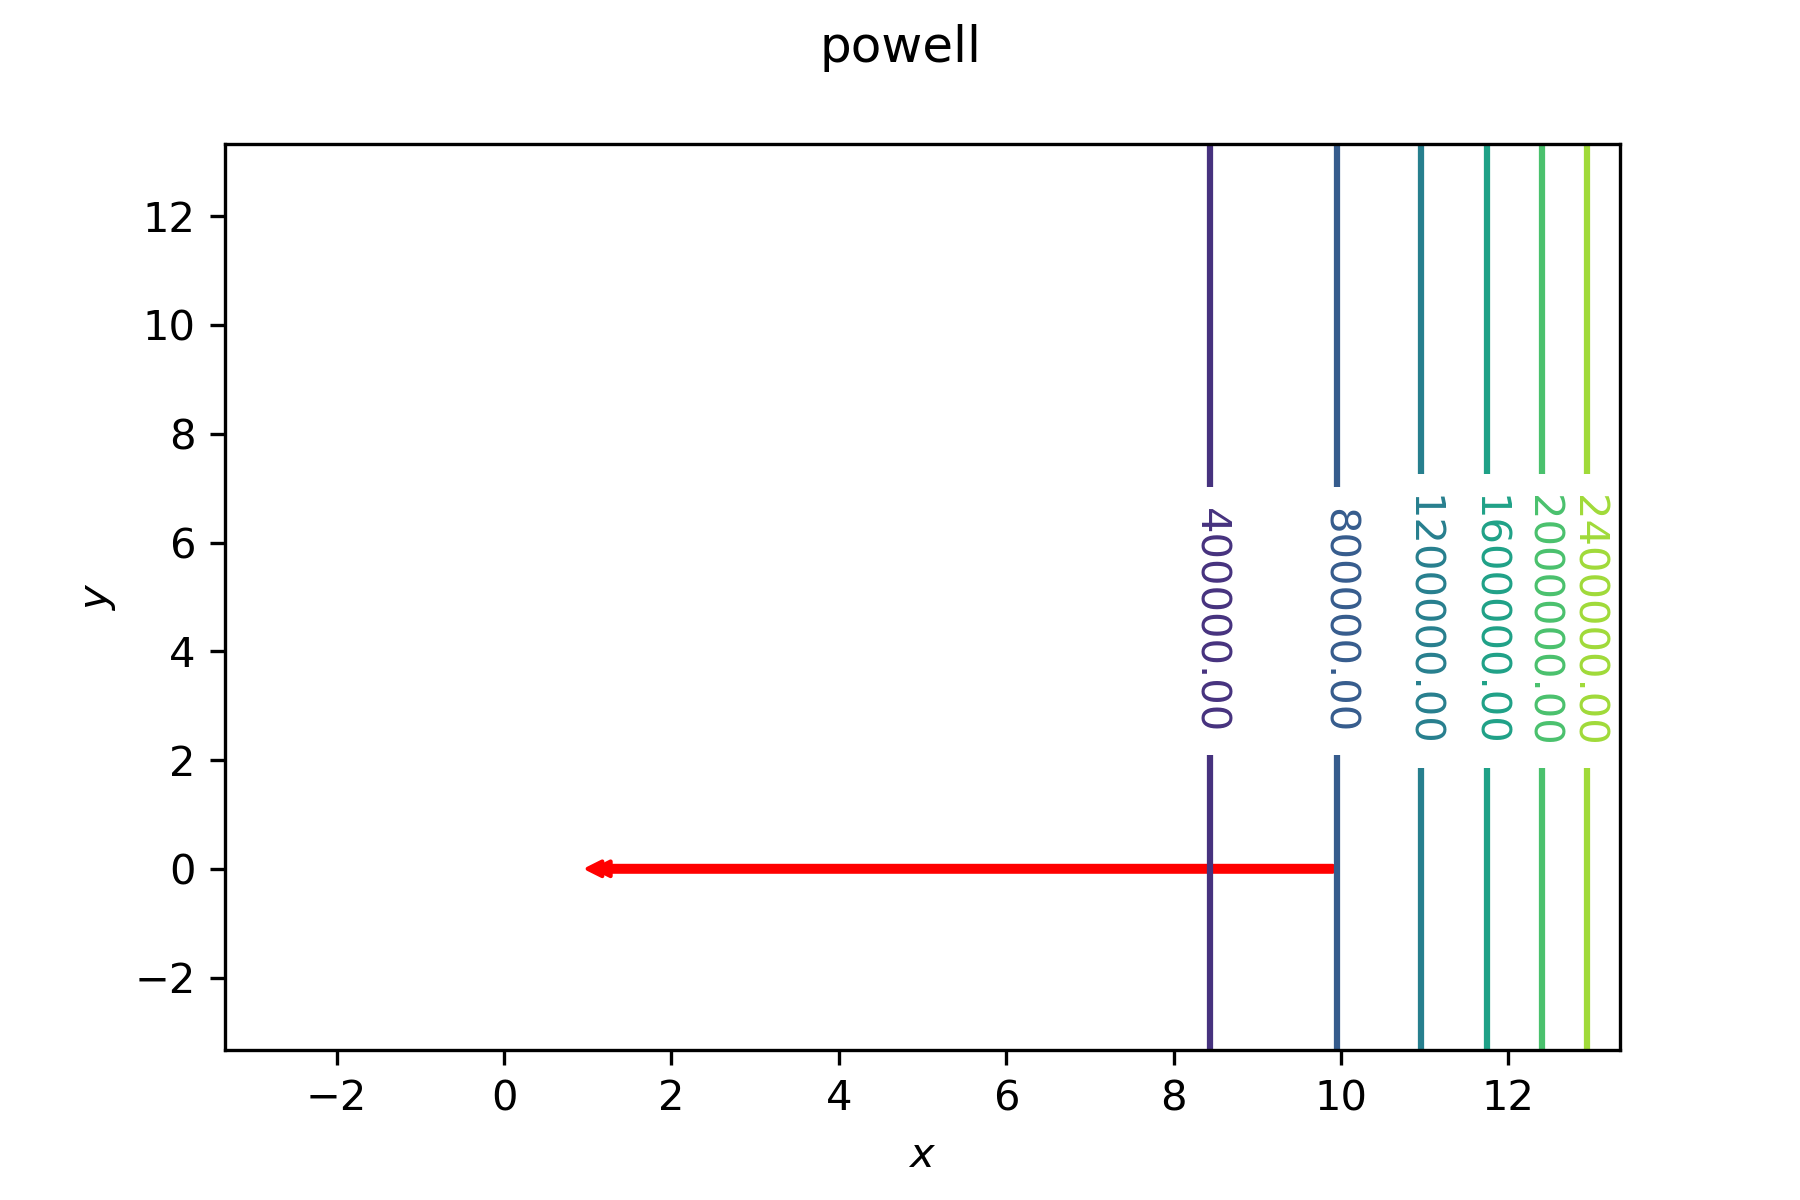
\includegraphics[scale=0.7]{plots/contours_powell_6.png}
\end{center}
\begin{center}
  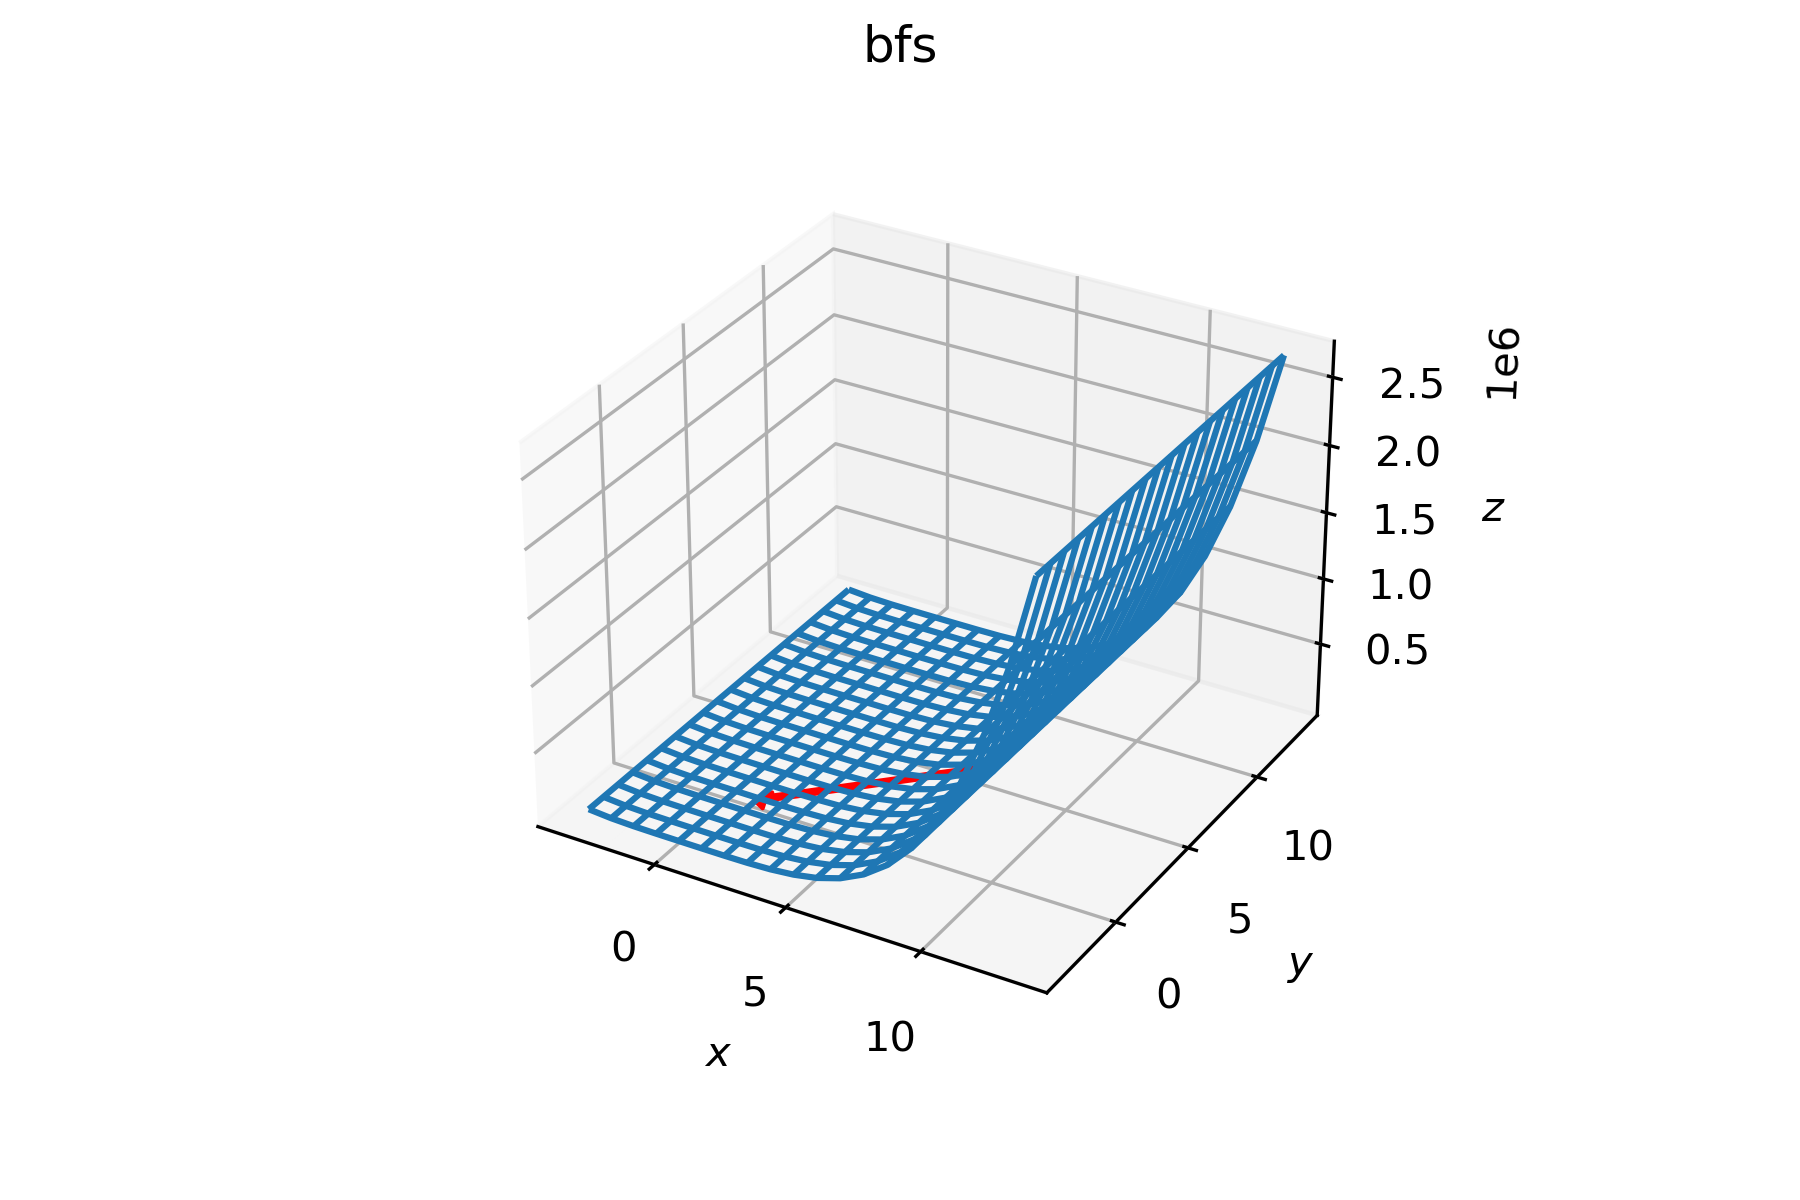
\includegraphics[scale=0.7]{plots/3D_bfs_6.png}
\end{center}
\begin{center}
  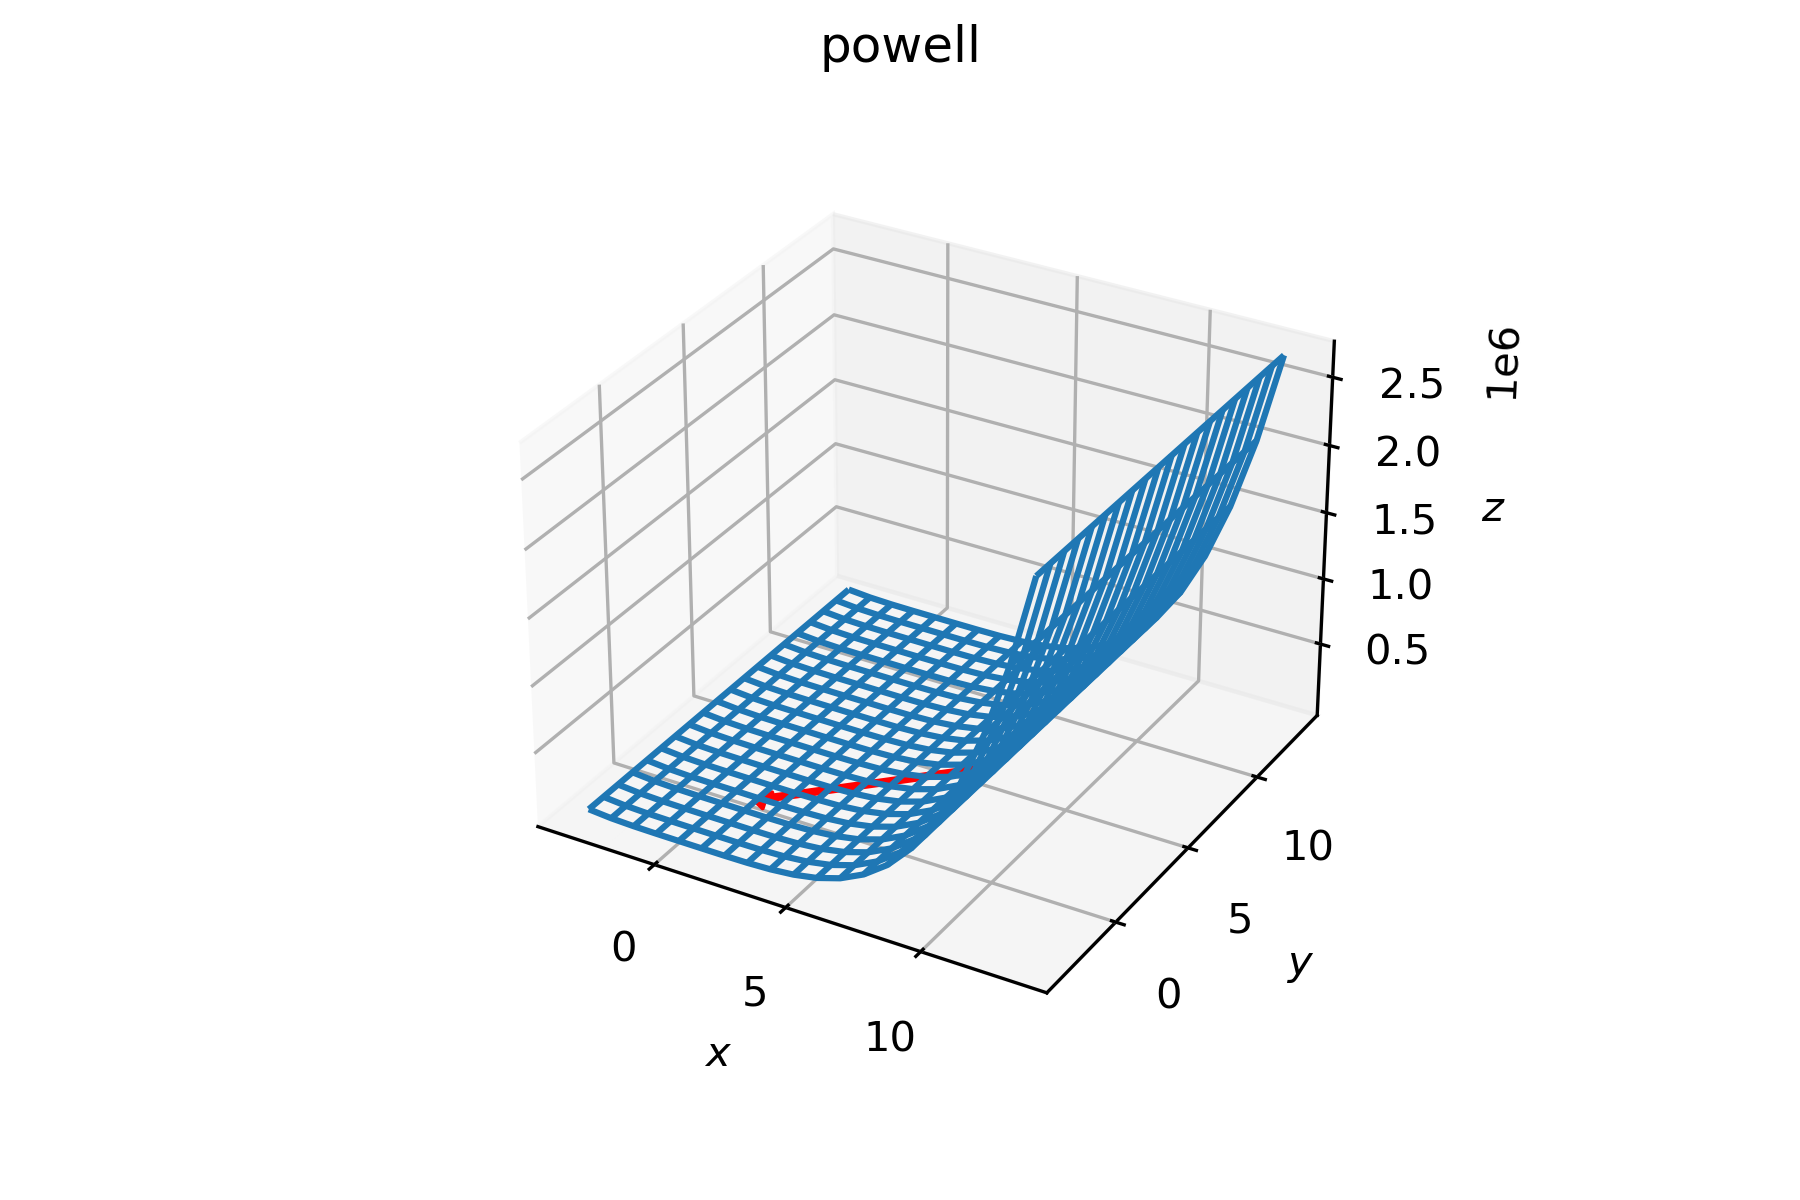
\includegraphics[scale=0.7]{plots/3D_powell_6.png}
\end{center}
\[ f_2(x) = (x_1^2 + x_2 - 11)^2 + (x_1 + x_2^2 - 7)^2 \quad x_0 = \begin{pmatrix}
  1 & 1
\end{pmatrix} \]
\begin{center}
  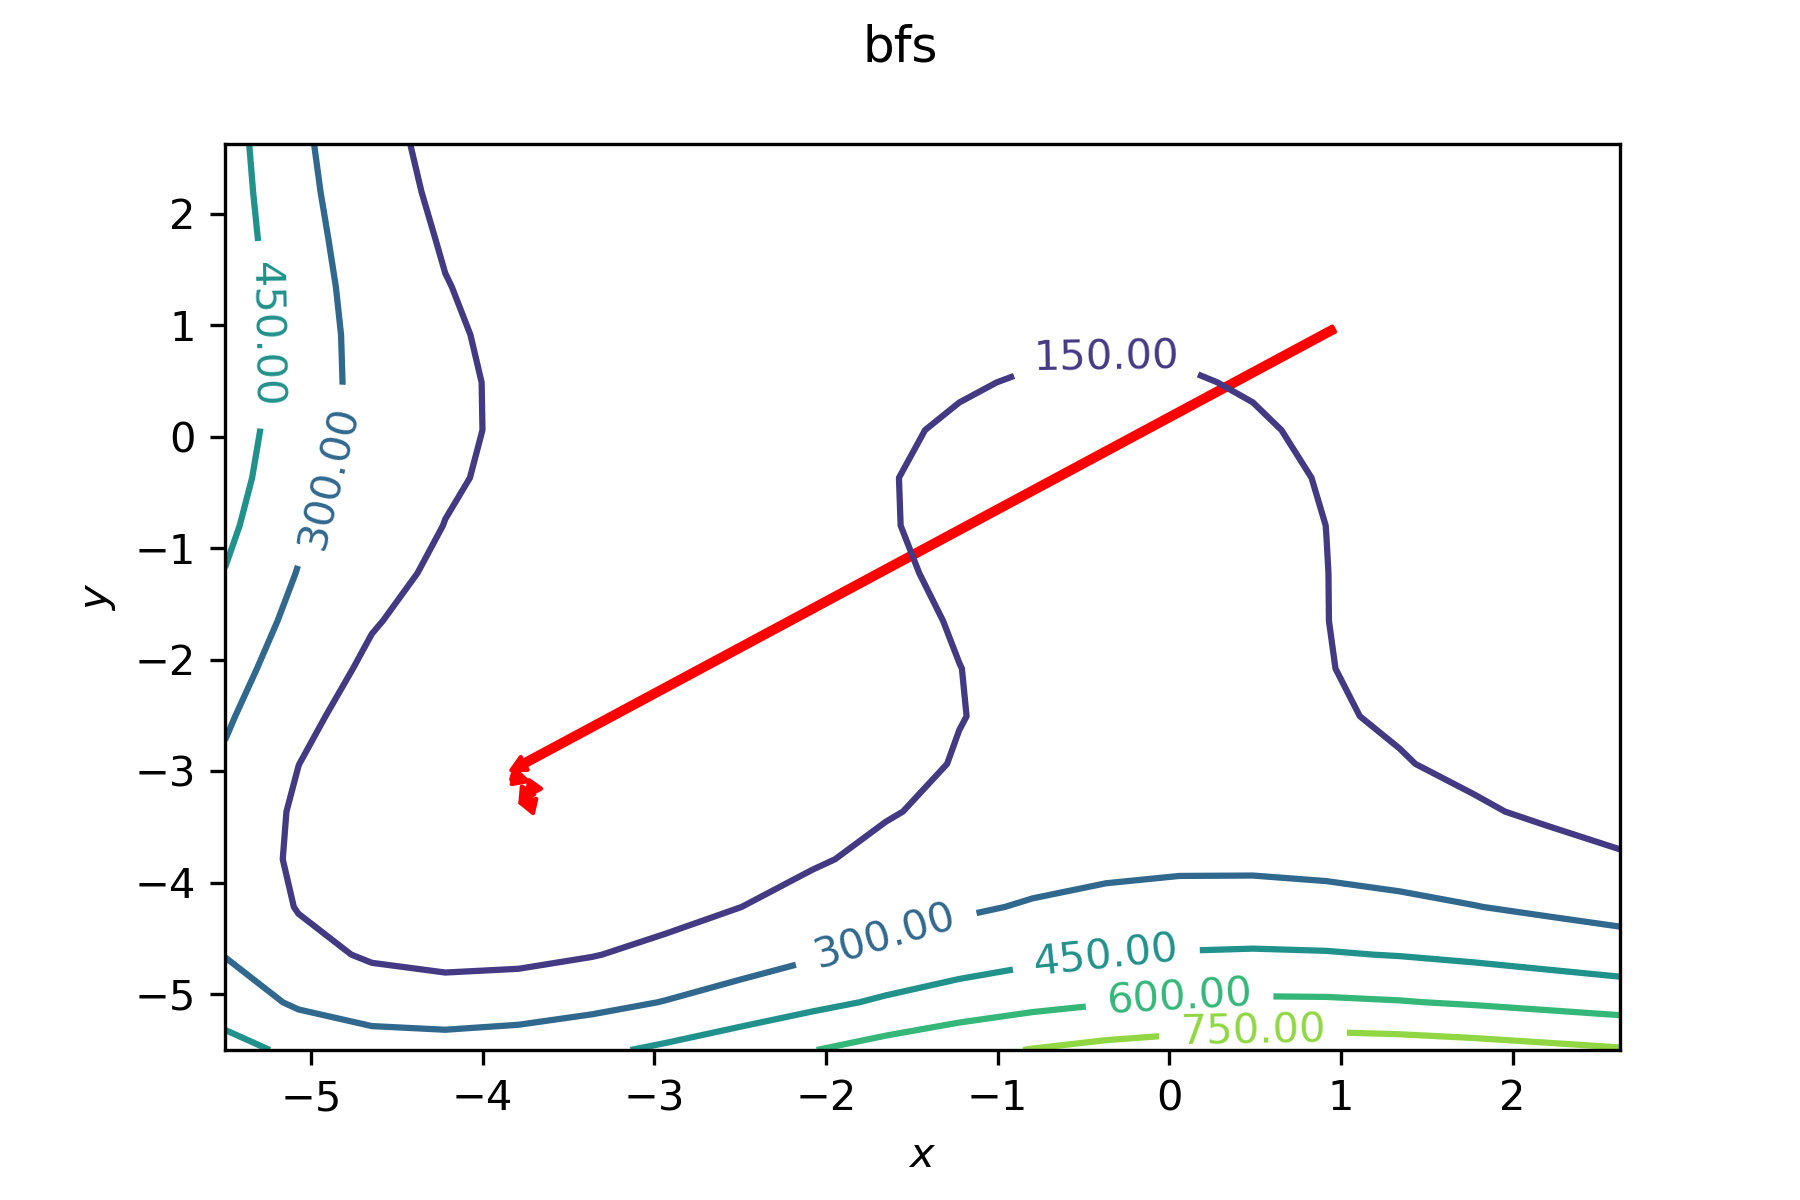
\includegraphics[scale=0.7]{plots/contours_bfs_7.png}
\end{center}
\begin{center}
  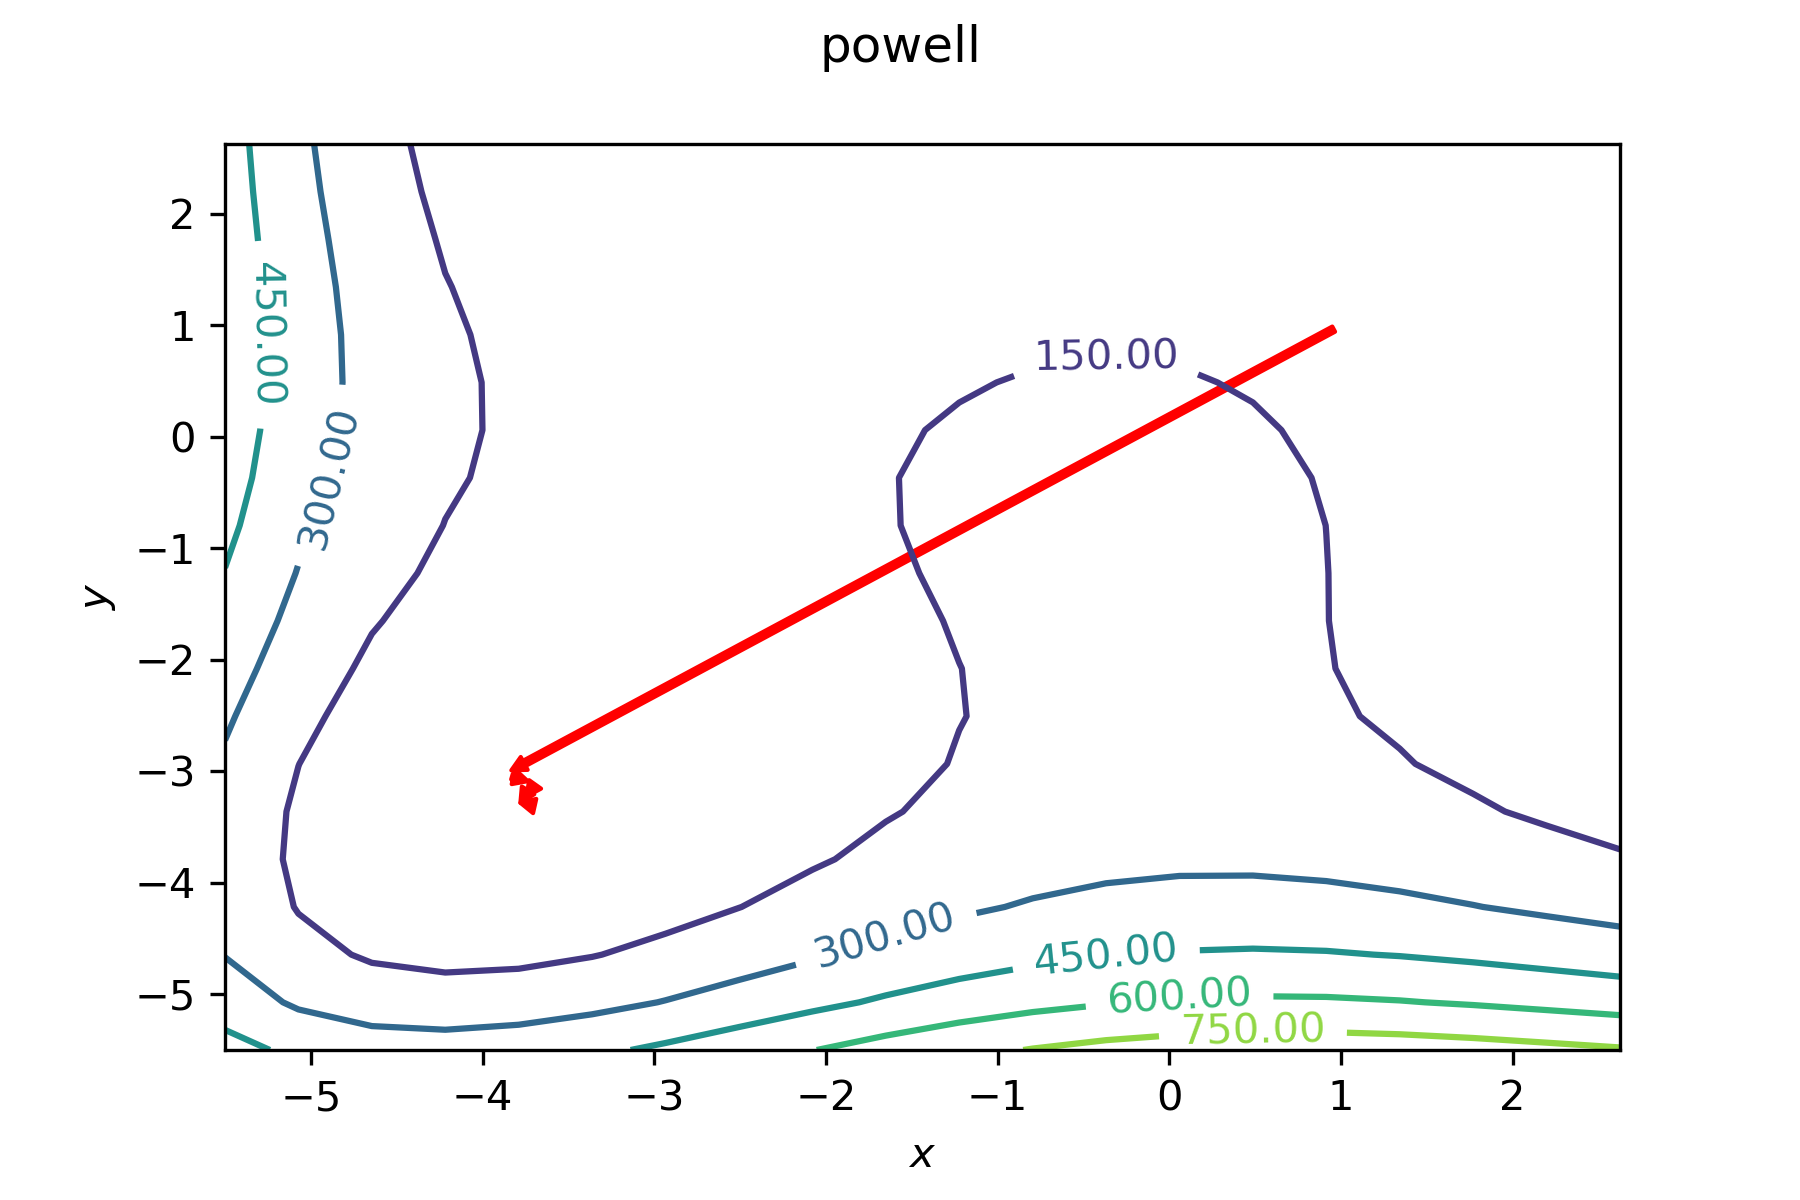
\includegraphics[scale=0.7]{plots/contours_powell_7.png}
\end{center}
\begin{center}
  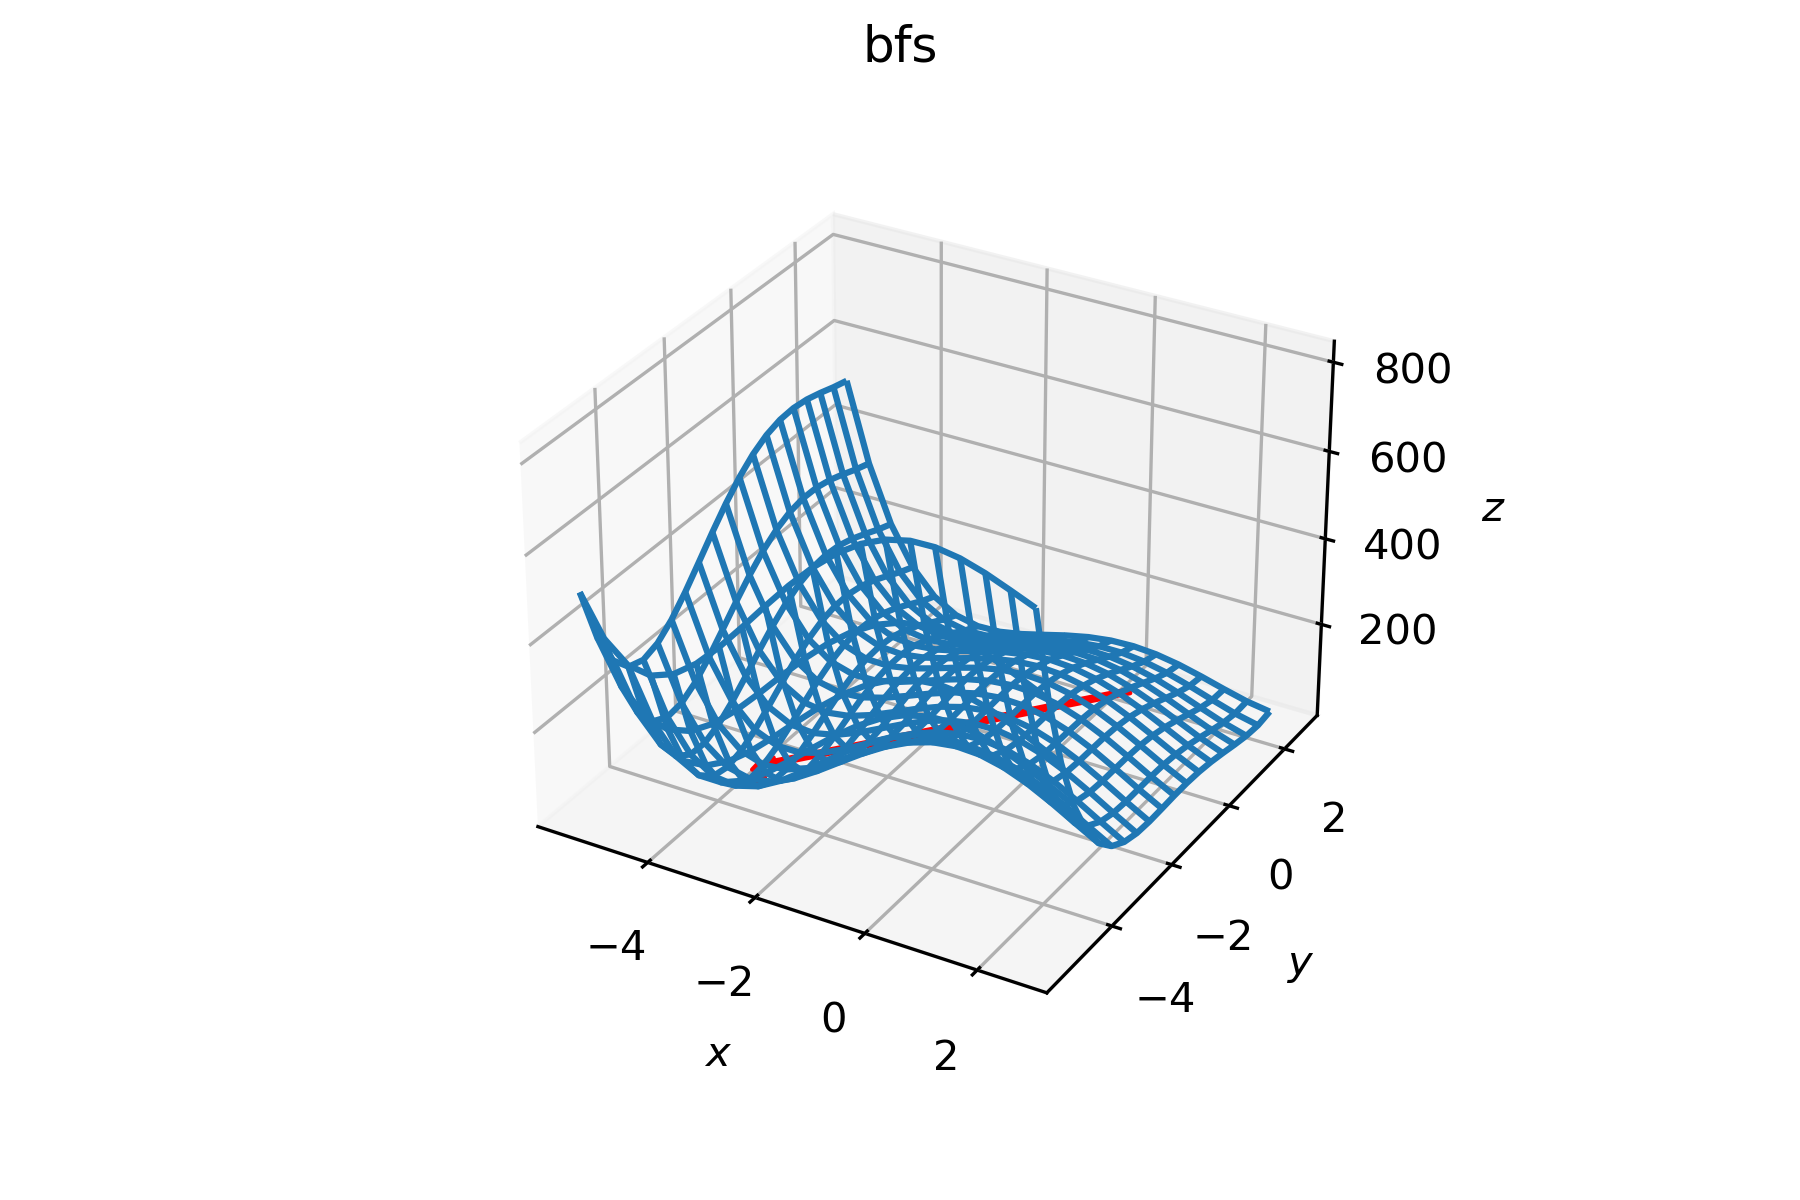
\includegraphics[scale=0.7]{plots/3D_bfs_7.png}
\end{center}
\begin{center}
  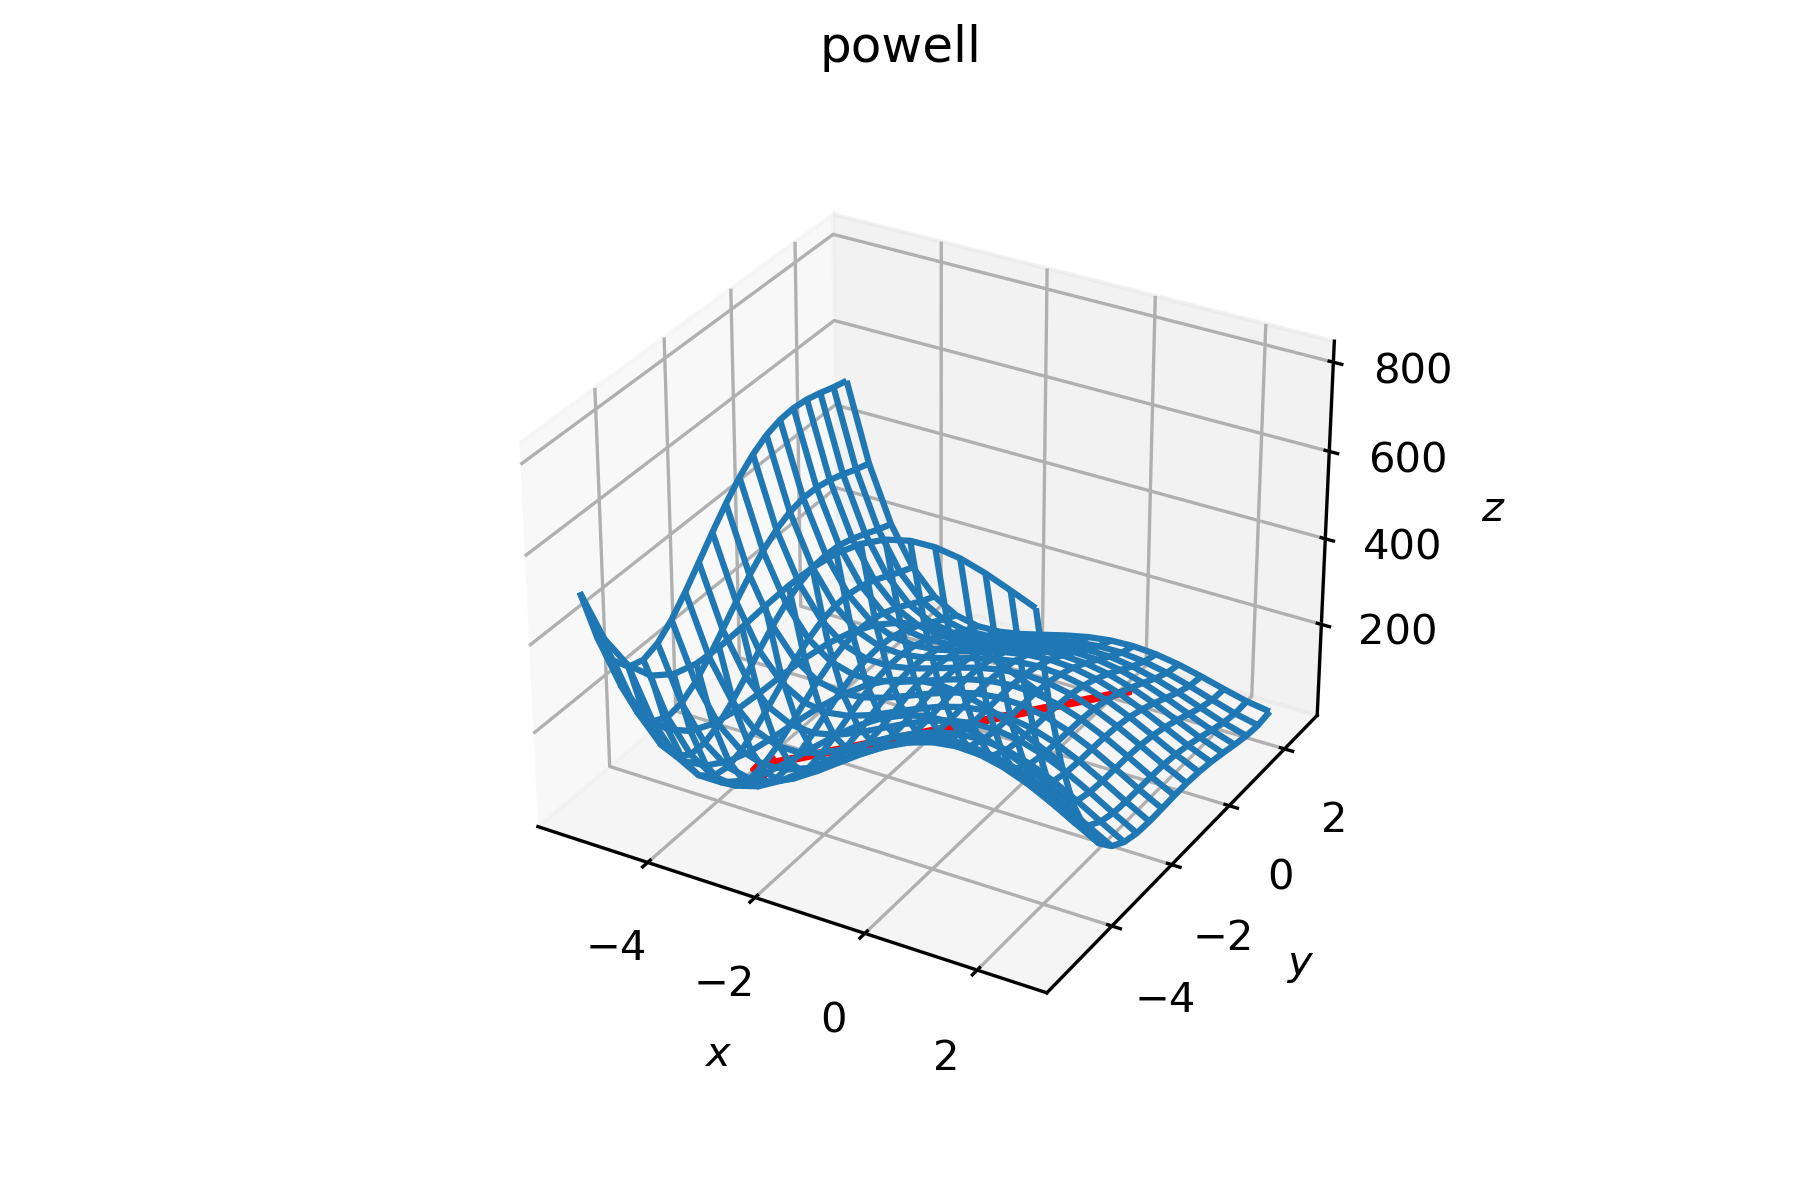
\includegraphics[scale=0.7]{plots/3D_powell_7.png}
\end{center}
\[ f_3(x) = (x_1 + 10x_2)^2 + 5(x_3 - x_4)^2 + (x_2 - 2x_3)^4 + 10(x_1 - x_4)^4 \]
\[ f_4(x) = 100 - \frac{2}{1 + \left(\frac{x_1 - 1}{2}\right)^2 + \left(\frac{x_2 - 1}{3}\right)^2} - \frac{1}{1 + \left(\frac{x_1 - 2}{2}\right)^2 + \left(\frac{x_2 - 1}{3}\right)^2} \quad x_0 = \begin{pmatrix}
  1, 1
\end{pmatrix}\]
\begin{center}
  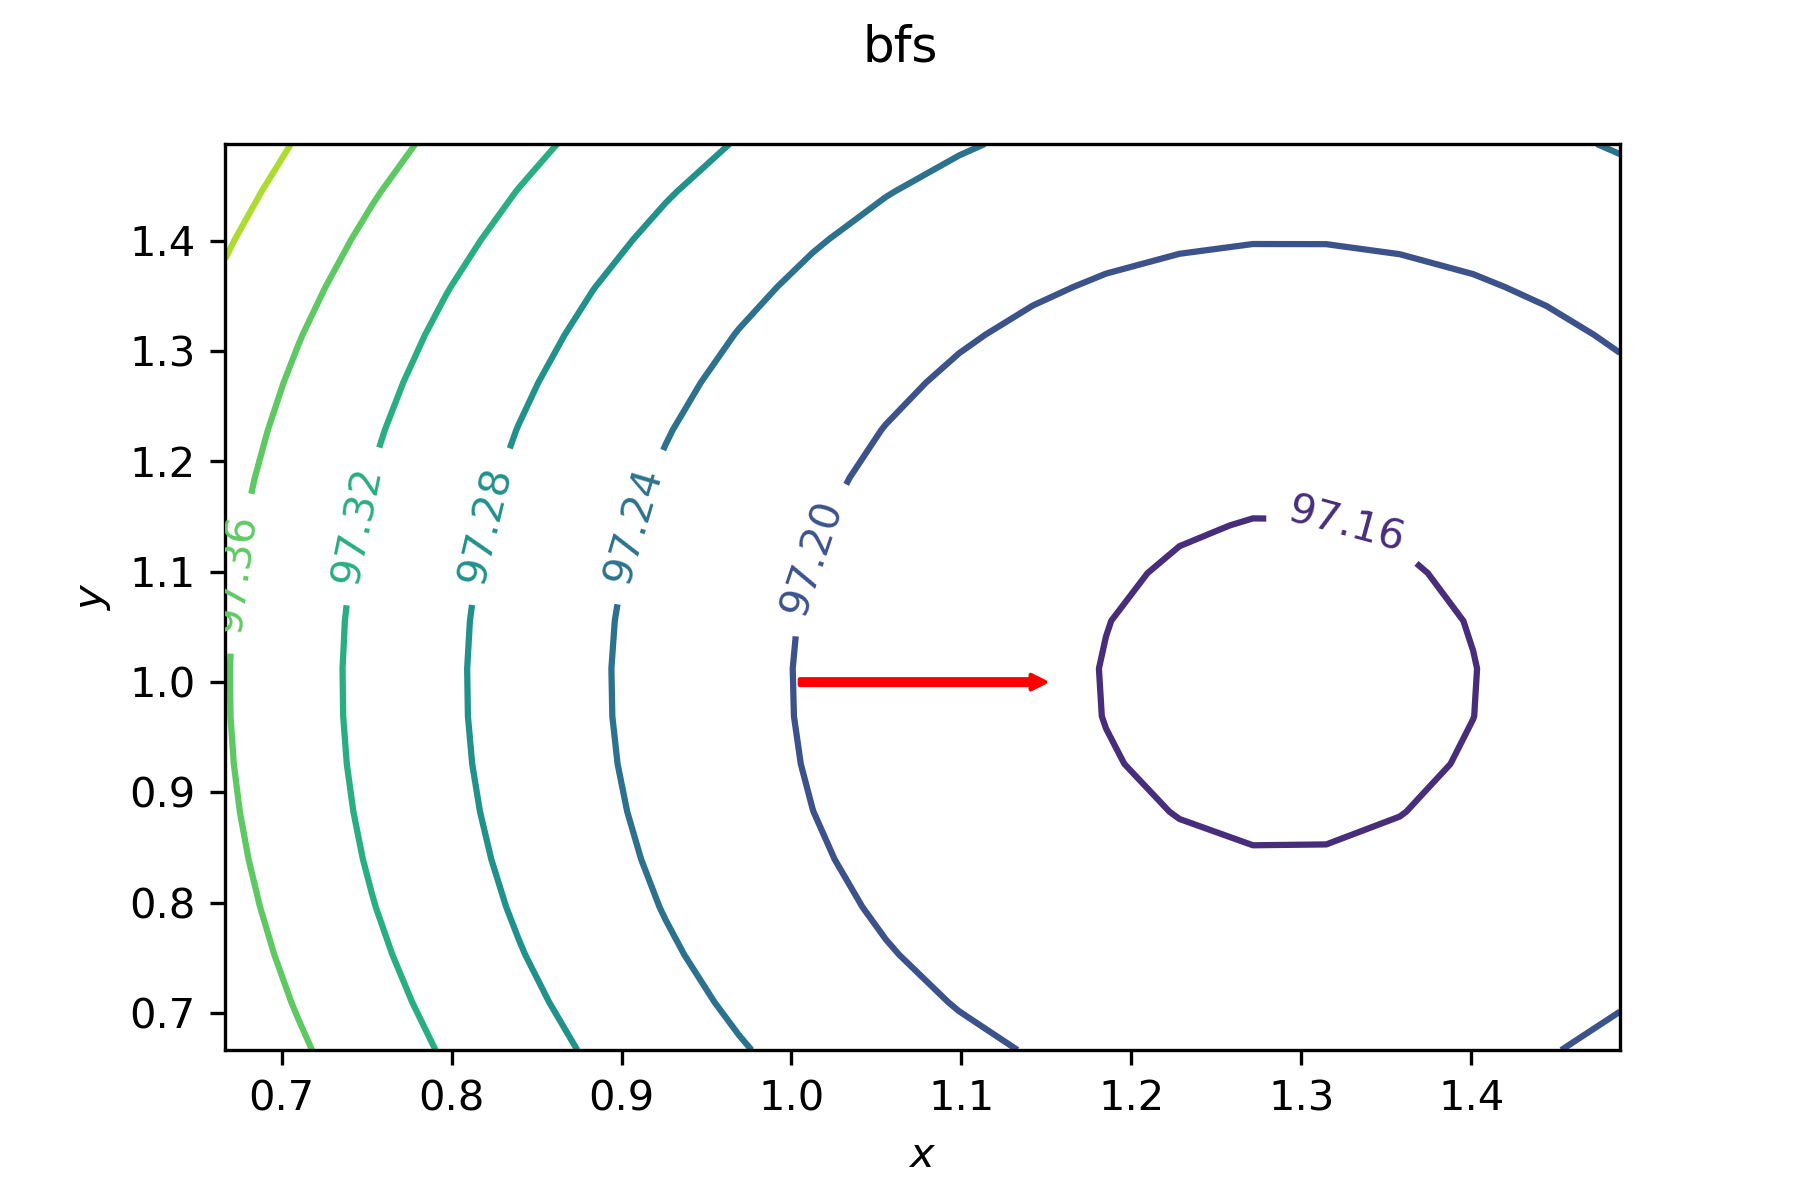
\includegraphics[scale=0.7]{plots/contours_bfs_9.png}
\end{center}
\begin{center}
  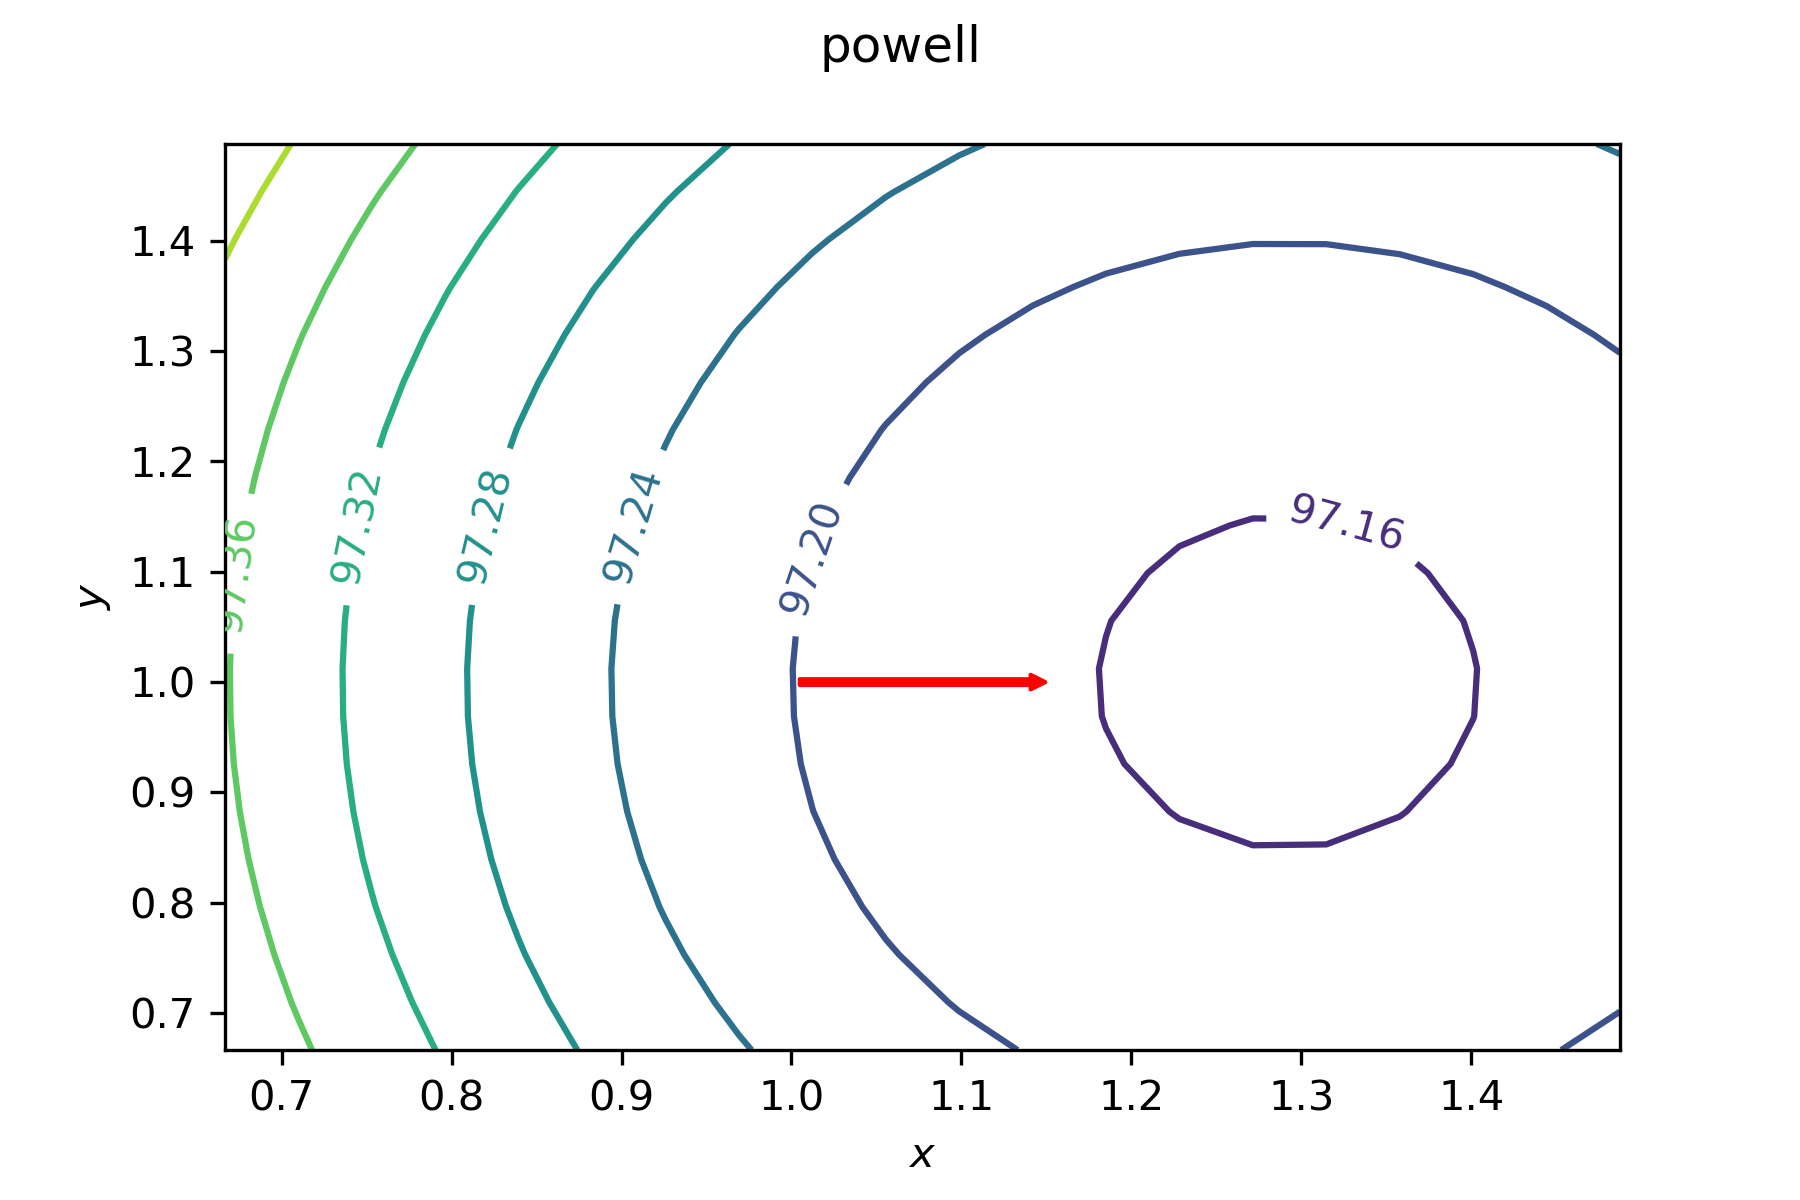
\includegraphics[scale=0.7]{plots/contours_powell_9.png}
\end{center}
Таблица количества итераций на представленных выше функциях и
соответствующих начальных приближениях (\(\infty\) обозначается, что
метод превысил максимальное количество итераций)
\begin{center}
  \begin{longtable}{l|cccc}
    Метод &  \(f_1\) & \(f_2\) & \(f_3\) & \(f_4\)\\
    \hline
    Бройдена-Флетчера-Шено & 3 & 7 & 16 & 3 \\
    \hline
    Пауэлла & 3 & 7 & 15 & 3 \\
    \hline
    Ньютона с направлением спуска & 2 & 5 & 18 & \(\infty\)
  \end{longtable}
\end{center}
Видно что на функция малой арности(2) наилучший из методов Ньютона
показывает немного меньшее число итераций, однако на функции \(f_3\)
квазиньютоновские методы показали себя лучше. На функции \(f_4\) метод
Ньютона застрял в одной точке и превысил максимально допустимое число
итераций, тогда как другие два метода сошлись к минимуму за 3 шага.


Таблица зависимости числа итераций от выбора начального приближения на функции \(f_2\) (она более разнообразна по сравнению с остальными).
\[ x_1 = \begin{pmatrix}
  1 & 1
\end{pmatrix} \quad x_2 = \begin{pmatrix}
  -1 & -3
\end{pmatrix} \quad x_3 = \begin{pmatrix}
  0 & 0
\end{pmatrix}\]
\begin{center}
  \begin{longtable}{l|ccc}
    Метод &  \(x_1\) & \(x_2\) & \(x_3\) \\
    \hline
    Бройдена-Флетчера-Шено &  7 & 11 & 9 \\
    \hline
    Пауэлла &  7 & 9 & 9 \\
  \end{longtable}
\end{center}
В точках \(x_1\) и \(x_3\) методы сходятся к минимума за одинаковое
количество итераций. При начальном приближении \(x_2\) метод Пауэлла
сходится немного быстрее.

Нельзя сказать, что какой-то метод работает лучше, они совершают
равное или примерно равное число итераций на различных функциях и
начальныз приближениях.
\section{Выводы}
В целом квазиньютоновские методы превосходят методы Ньютона по всем параметрам:
\begin{itemize}
\item Они совершают меньшее число итераций на похожих функциях и начальных приближения
\item Одно из главных их достоинств в том, что на многих функциях, где
  в методах Ньютона не существует решения СЛАУ, квазиньютоновские
  методы не имеют этого недостатка, так как не вычисляют матрицу
  \(H^{-1}\) напрямую, а используют приближенные вычисления, что
  однако не сказывается на точности.
\end{itemize}
\end{document}
